\section{Основы микропрограммного управления}
\label{ch::practice::programming}

Множительное устройство, ЦУУ и другие модули (см. рисунок \ref{fig::ch::practice::model}) работают автономно и каждый выполняет собственный алгоритм функционирования. Например, УЧ множительного устройства в бесконечном цикле выполняет алгоритм: принять задания от ЦУУ; выполнить умножение; выдать в ЦУУ результаты. ЦУУ, например, выполняет в бесконечном цикле алгоритм: считать очередную команду программы пользвателя из памяти; декодировать её; выдать необходимые задания исполнительным модулям; дождаться результатов, считать и сохранить их; выбрать следующую команду\ldots

УЧ модуля (в том числе и множительного устройства) представляет собой автомат, по тактам выполняющий алгоритм работы модуля. Существует несколько способов создания таких автоматов. В данном разделе будут рассморены математические основы функционирования управляющих автоматов, а затем особый вид таких автоматов --- \emph{микропрограммные}.

В математической основе выделяют два типа управляющих автоматов: автоматы Мили и автоматы Мура. Общим для автоматов обоих типов является:
\begin{itemize}
    \item Внутреннее состояние. Автомат в течение такта находится в одном из множества возможных внутренних состояний. По завершении такта, автомат переключается в новое состояние. Множество внутренних состояний 
    \[ 
        S=\{s_0,\ldots,s_{n-1}\}.
    \]
    
    \item Начальное состояние $s_0$. С этого внутреннего состояния автомат начинает свою работу.
    
    \item Набор значений (вектор) осведомительных сигналов
    \[
        P=(p_{m-1},\ldots,p_0).
    \]
	
	Новое внутреннее состояние, в которое перейдет автомат, определяется его текущим внутренним состоянием и значениями осведомительных сигналов, которые поступали ему в течение такта.
    
    
    \item Набор управляющих сигналов
    \[
        Y=(y_{k-1},\ldots,y_0).
    \]
	
	Автомат в течение такта формирует и выдает значения управляющих сигналов. В способе формирования  управляющих сигналов заключается главное отличие между автоматами Мили и Мура.
\end{itemize}

Если в $i$-м такте автомат находится в состоянии $s^{(i)}$, и поступают значения осведомительных сигналов $P^{(i)}$, то состояние $s^{(i+1)}$, в которое он перейдет в следующем такте, определяется функцией перехдов $\mathbf{S}$, а набор управляющих сигналов, которые выдаются в $i$-м такте $Y^{(i)}$ определяются функцией выходов $\mathbf{Y}$.

Для автомата Мили:
\begin{equation}
    \begin{aligned}
        s^{(i+1)}&=\mathbf{S}(s^{(i)}, P^{(i)});\\
        Y^{(i)}  &=\mathbf{Y}(s^{(i)}, P^{(i)}).
    \end{aligned}
    \label{eq::ch::practice::programming::Mili}
\end{equation}

Видно, что для автомата Мили векор управляющих сигналов $Y^{(i)}$ формируется на основе текущего состояния $s^{(i)}$ и вектора осведомительных сигналов $P^{(i)}$.

Для автомата Мура управляющие сигналы зависят только от текущего состояния:
\begin{equation}
    \begin{aligned}
        s^{(i+1)}&=\mathbf{S}(s^{(i)}, P^{(i)});\\
        Y^{(i)}  &=\mathbf{Y}(s^{(i)}).
    \end{aligned}
    \label{eq::ch::practice::programming::Moore}
\end{equation}

Работу автомата удобно изобразить на диаграмме переходов, которая представляет собой граф, вершинам которого соответствуют состояния, а дугам --- функция переходов $\mathbf{S}$. Начальное состояние $s_0$ обычно выделяется двойным контуром. Над дугой подписываются значения осведомительных сигналов, определяющих переход в следующее состояние. Так как управляющие сигналы в автомате Мили зависят от состояния автомата и осведомительных сигналов, то управляющими сигналами взвешиваются дуги. В автомате Мура управляющие сигналы зависят только от состояния, поэтому управляющими сигналами взвешиваются вершины.

Далее приводятся примеры диаграмм переходов автоматов, из раздела \ref{ss::ch::practice::software::example}, к этому разделу следует обратиться всем желающим понять назначение управляющих и осведомительных сигналов. Пока же --- это неважно.

\begin{figure}[!ht]
    \[
        {\xymatrix{
            *{}
                &*{}
                    &*{}
                        &s_3  \ar@{->}@/^/[dr]^(.3){*|\Machine{22h}} 
                            &*{}
                                &*{}
                                    &*{}
                                        &*{}
                                            \\
            *++[o][F=]{s_0}  \ar@{->}[r]^{p_0|\Machine{1h}}  \ar@{->}@(ur,ul)[]_{\bar{p}_0|\Machine{1h}}
                &s_1  \ar@{->}[r]^{*|\Machine{4h}}
                    &s_2  \ar@{->}[rr]^{\bar{p}_2|\Machine{12h}} \ar@{->}@/^/[ur]^{p_2|\Machine{18h}}
                        &*{}
                            &s_4  \ar@{->}[rr]^{p_1|\Machine{2h}} \ar@{->}@(r,u)[]_(.6){\bar{p}_1|\Machine{2h}}
                                &*{}
                                    &s_5  \ar@{->}@(d,d)[llllll]_{*|\Machine{41h}}
        }}
    \]
    \caption{Диаграмма переходов автомата Мили}
    \label{fig::ch::practice::MiliDiagram}
\end{figure}

На рисунке \ref{fig::ch::practice::MiliDiagram} приведена диаграмма автомата Мили. Далее приводится описание нескольких переходов.
\begin{itemize}
    \item Из начального состояния $s_0$, автомат переходит в состояние $s_1$, при $p_0=1$ (на схеме это обозначено как $p_0$); при этом выдается управляющий сигнал $y_0$ (на схеме вектор управляющих сигналов закодирован в 16-ичной СС: \Machine{1h}).
    
    \item Автомат остается в начальном состояниии если $\bar{p}_0$, при этом также выдается $y_0$.

    \item Из $s_1$ осуществляется переход только в $s_2$ --- осведомительные сигналы не важны (переход помечен $*$), при этом выдается управляющий сигнал $y_2$ (вектор \Machine{4h}).
    
    \item Из $s_5$ автомат безусловно возвращается в $s_0$ и выдает при этом набор сигналов $\{y_6,y_0\}$, т.е. вектор \Machine{41h}.
\end{itemize}

Из состояния $s_1$ автомат переходит только в состояние $s_2$, при этом значения осведомительных сигналов не важны и обозначены на схеме $*$, выдается управляющий сигнал $y_0$. И т.д.

\begin{figure}[!ht]
    \[
        {\xymatrix{
            *{} &*{}&*{}&*{}&*{}&*{}&*{}    \\
            *{}
                &*{}
                    &*{}
                        &s_5|\Machine{10h}    \ar@{->}@/^/[rrd]^{*} 
                            &*{}
                                &*{}
                                    &*{}
                                        \\
            *++[o][F=]{s_0|\Machine{1h}}  \ar@{->}[r]^{p_0}  \ar@{->}@(ur,ul)[]_{\bar{p}_0}
                &s_1|\Machine{4h}  \ar@{->}[r]^{*}
                    &s_2|\Machine{0h}  \ar@{->}[r]^{p_2}  \ar@{->}@/^/[ru]^{\bar{p}_2}
                        &s_3|\Machine{18h}  \ar@{->}[r]^{*}
                            &s_4|\Machine{20h}  \ar@{->}[r]^{*}
                                &s_6|\Machine{2h}  \ar@{->}[r]^{p_1} \ar@{->}@(ur,ul)[]_{\bar{p}_1}
                                    &s_7|\Machine{41h} \ar`d[dl]`_u[llllll]_{\bar{p}_0}[llllll]
                                                       \ar`u[uul]`[lllll]_{p_0}[lllll]
                                        %\ar@{->}@(d,d)[llllll]_{\bar{p}_0} \ar@{->}@(u,u)[lllll]_{p_0}
                                            \\
            *{} &*{}&*{}&*{}&*{}&*{}&*{}    \\
        }}
    \]
    \caption{Диаграмма переходов автомата Мура}
    \label{fig::ch::practice::MooreDiagram}
\end{figure}

На рисунке \ref{fig::ch::practice::MooreDiagram} приведена диаграмма автомата Мура. Далее следует описания нескольких переходов автомата.
\begin{itemize}
    \item Находясь в начальном состоянии, автомат выдает управлающий сигнал $y_0$ (вектор \Machine{1h}). Если выполняется условие $\bar{p}_0$, т.е. $p_0=0$, то автомат остается в начальном состоянии, в противном случае --- переходит в $s_1$.
    
    \item Из состояния $s_3$, в котором автомат выдает управляющие сигналы $\{y_4,y_3\}$, автомат безусловно переходит в $s_4$.
    
    \item Из состояния $s_5$ автомат может вернуться в начальное состояние или выполнить переход в $s_0$.
\end{itemize}

\emph{Микропрограммный} автомат в своем составе имеет два элемента --- микропроцессор и память \emph{микрокоманд}. Такие автоматы довольно удобны в обращении, так как позволяют задать алгоритм своей работы простой записью микропрограммы в память микрокоманд. Микрокоманда выполняется за один такт и сопровождается выдачей соответствующих управляющих сигналов.


\subsection{Микропрограммные автоматы}

Структура микропрограммного автомата Мили представлена на рисунке\footnote{Мы намеренно отступили от некоторых правил оформления схем --- например, мультиплексор MS1 в нашей схеме перевернут, а управление на MS2 подается слева} \ref{fig::ch::practice::Mili}, а Мура --- на рисунке \ref{fig::ch::practice::Moore}. 

\begin{figure}[!ht]
    \centering
    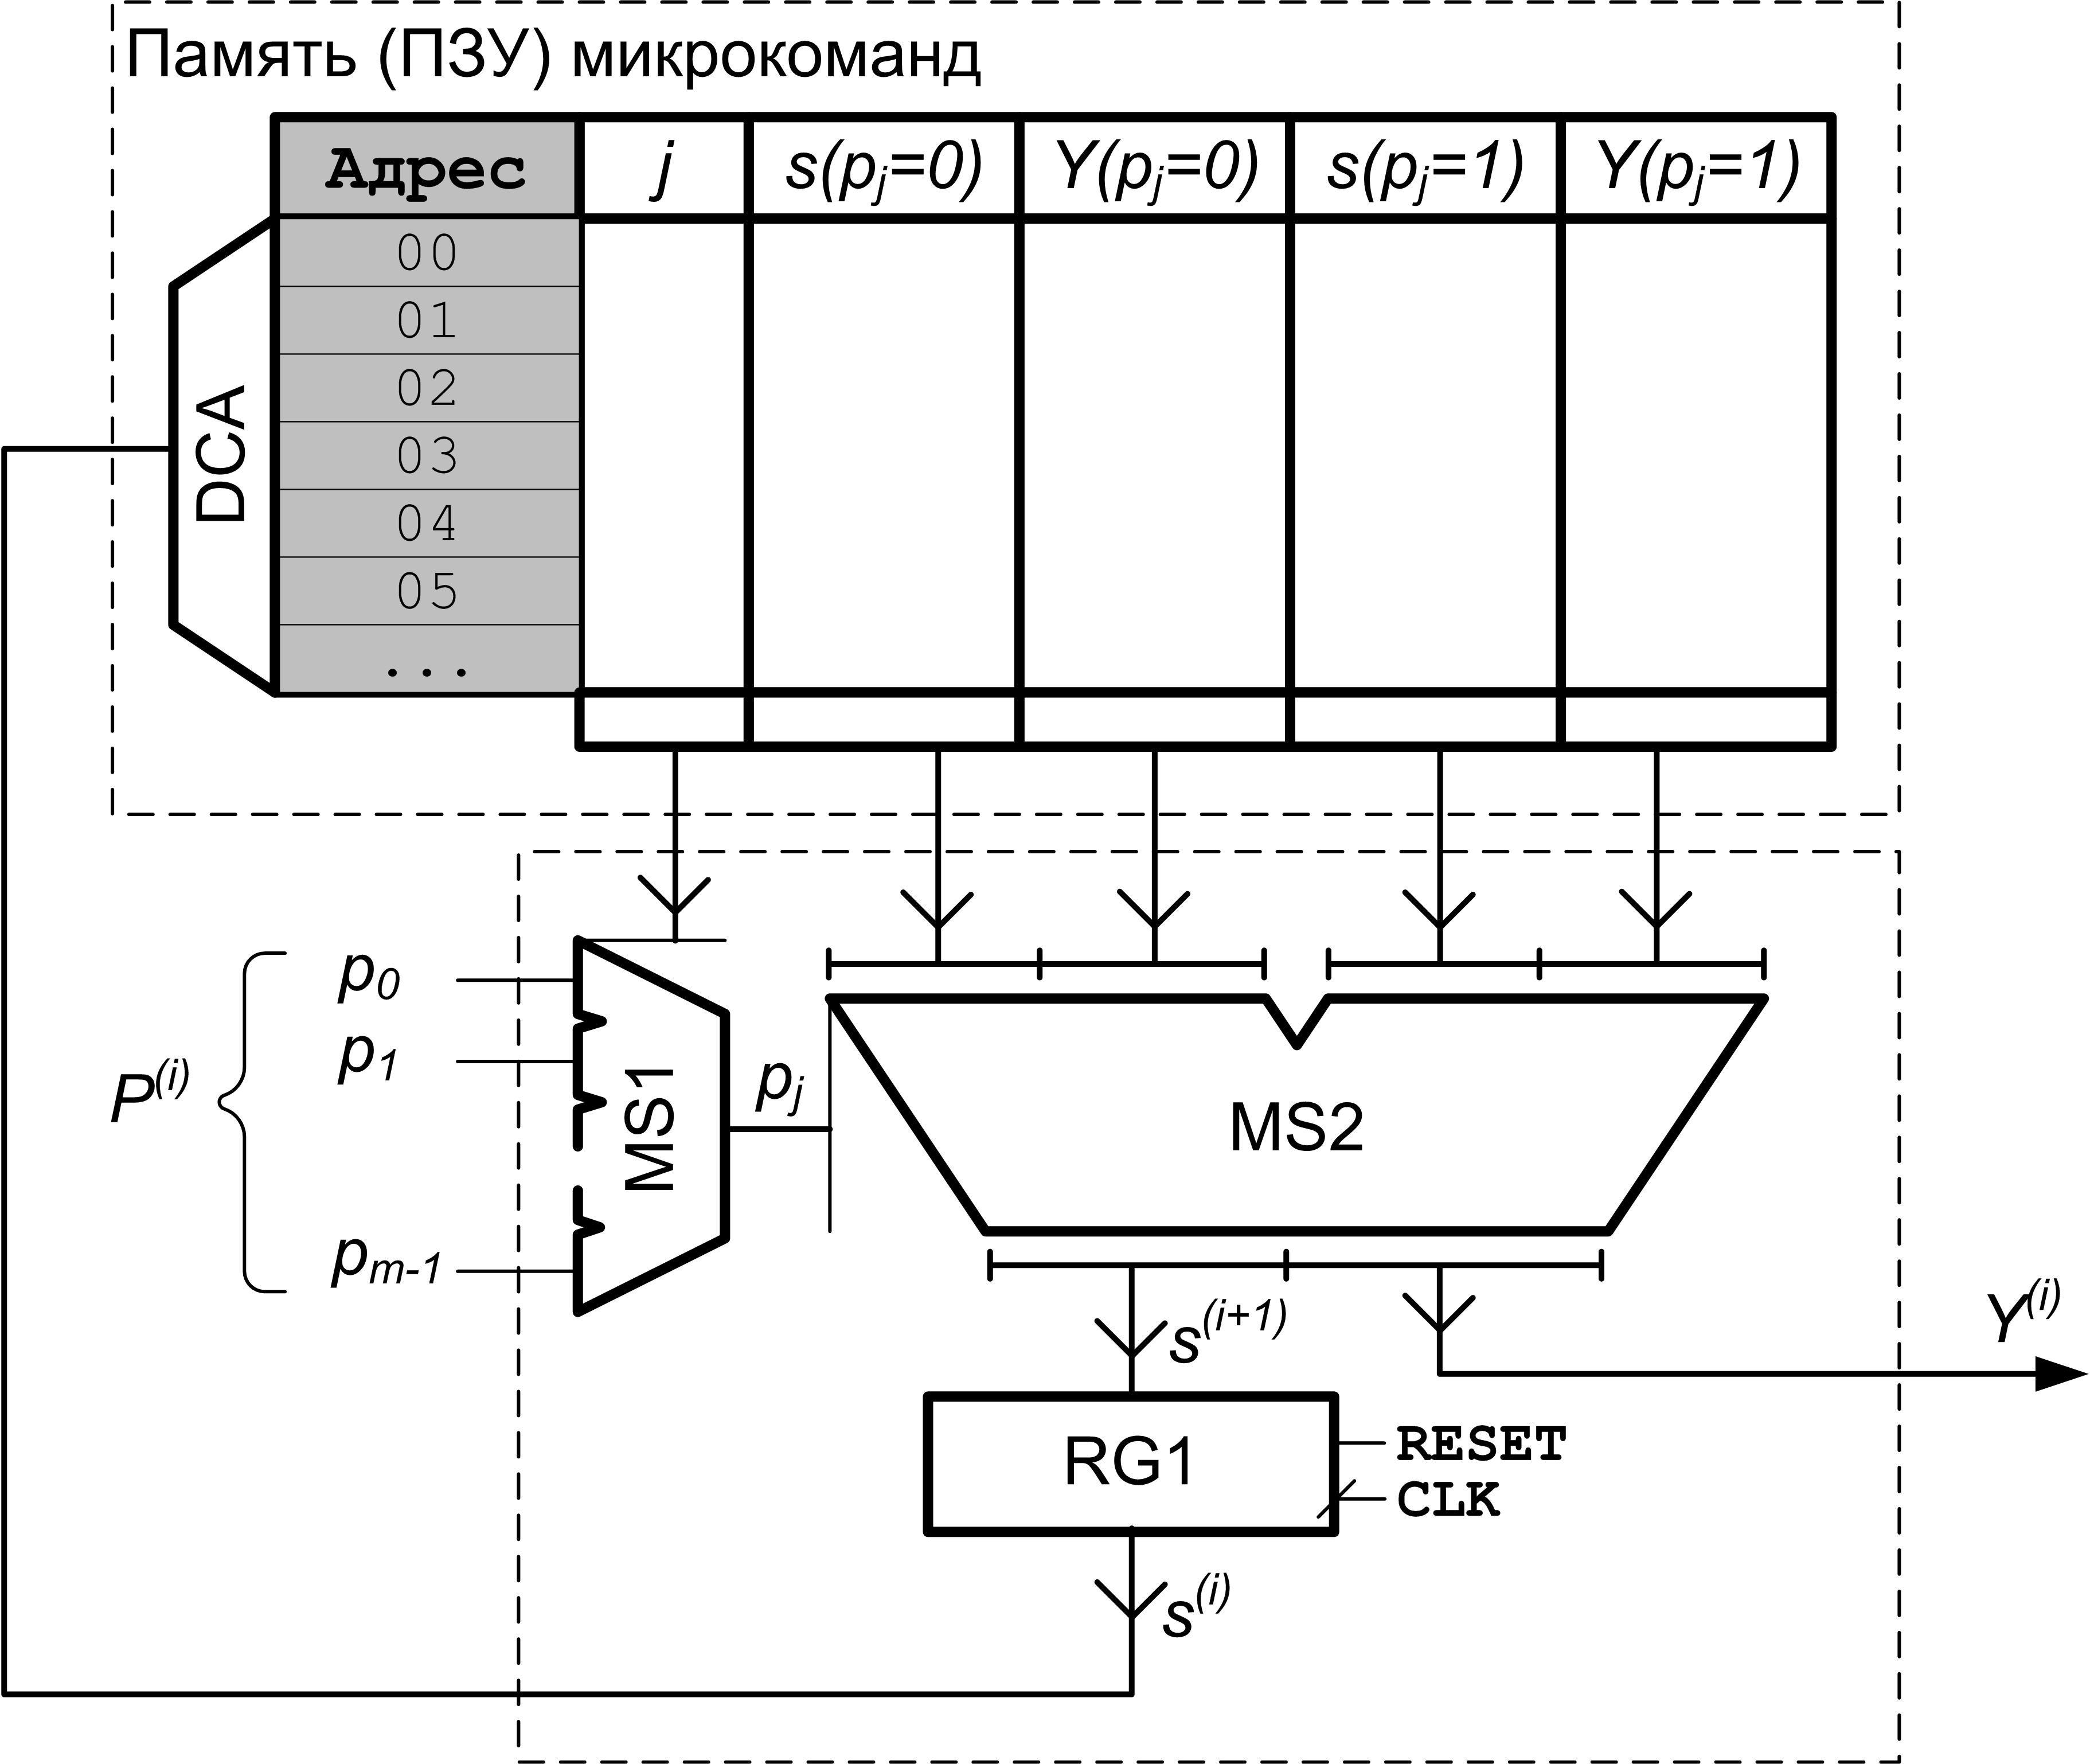
\includegraphics{fig/mili} 
    \caption{Автомат Мили}
    \label{fig::ch::practice::Mili}
\end{figure}

\begin{figure}[!ht]
    \centering
    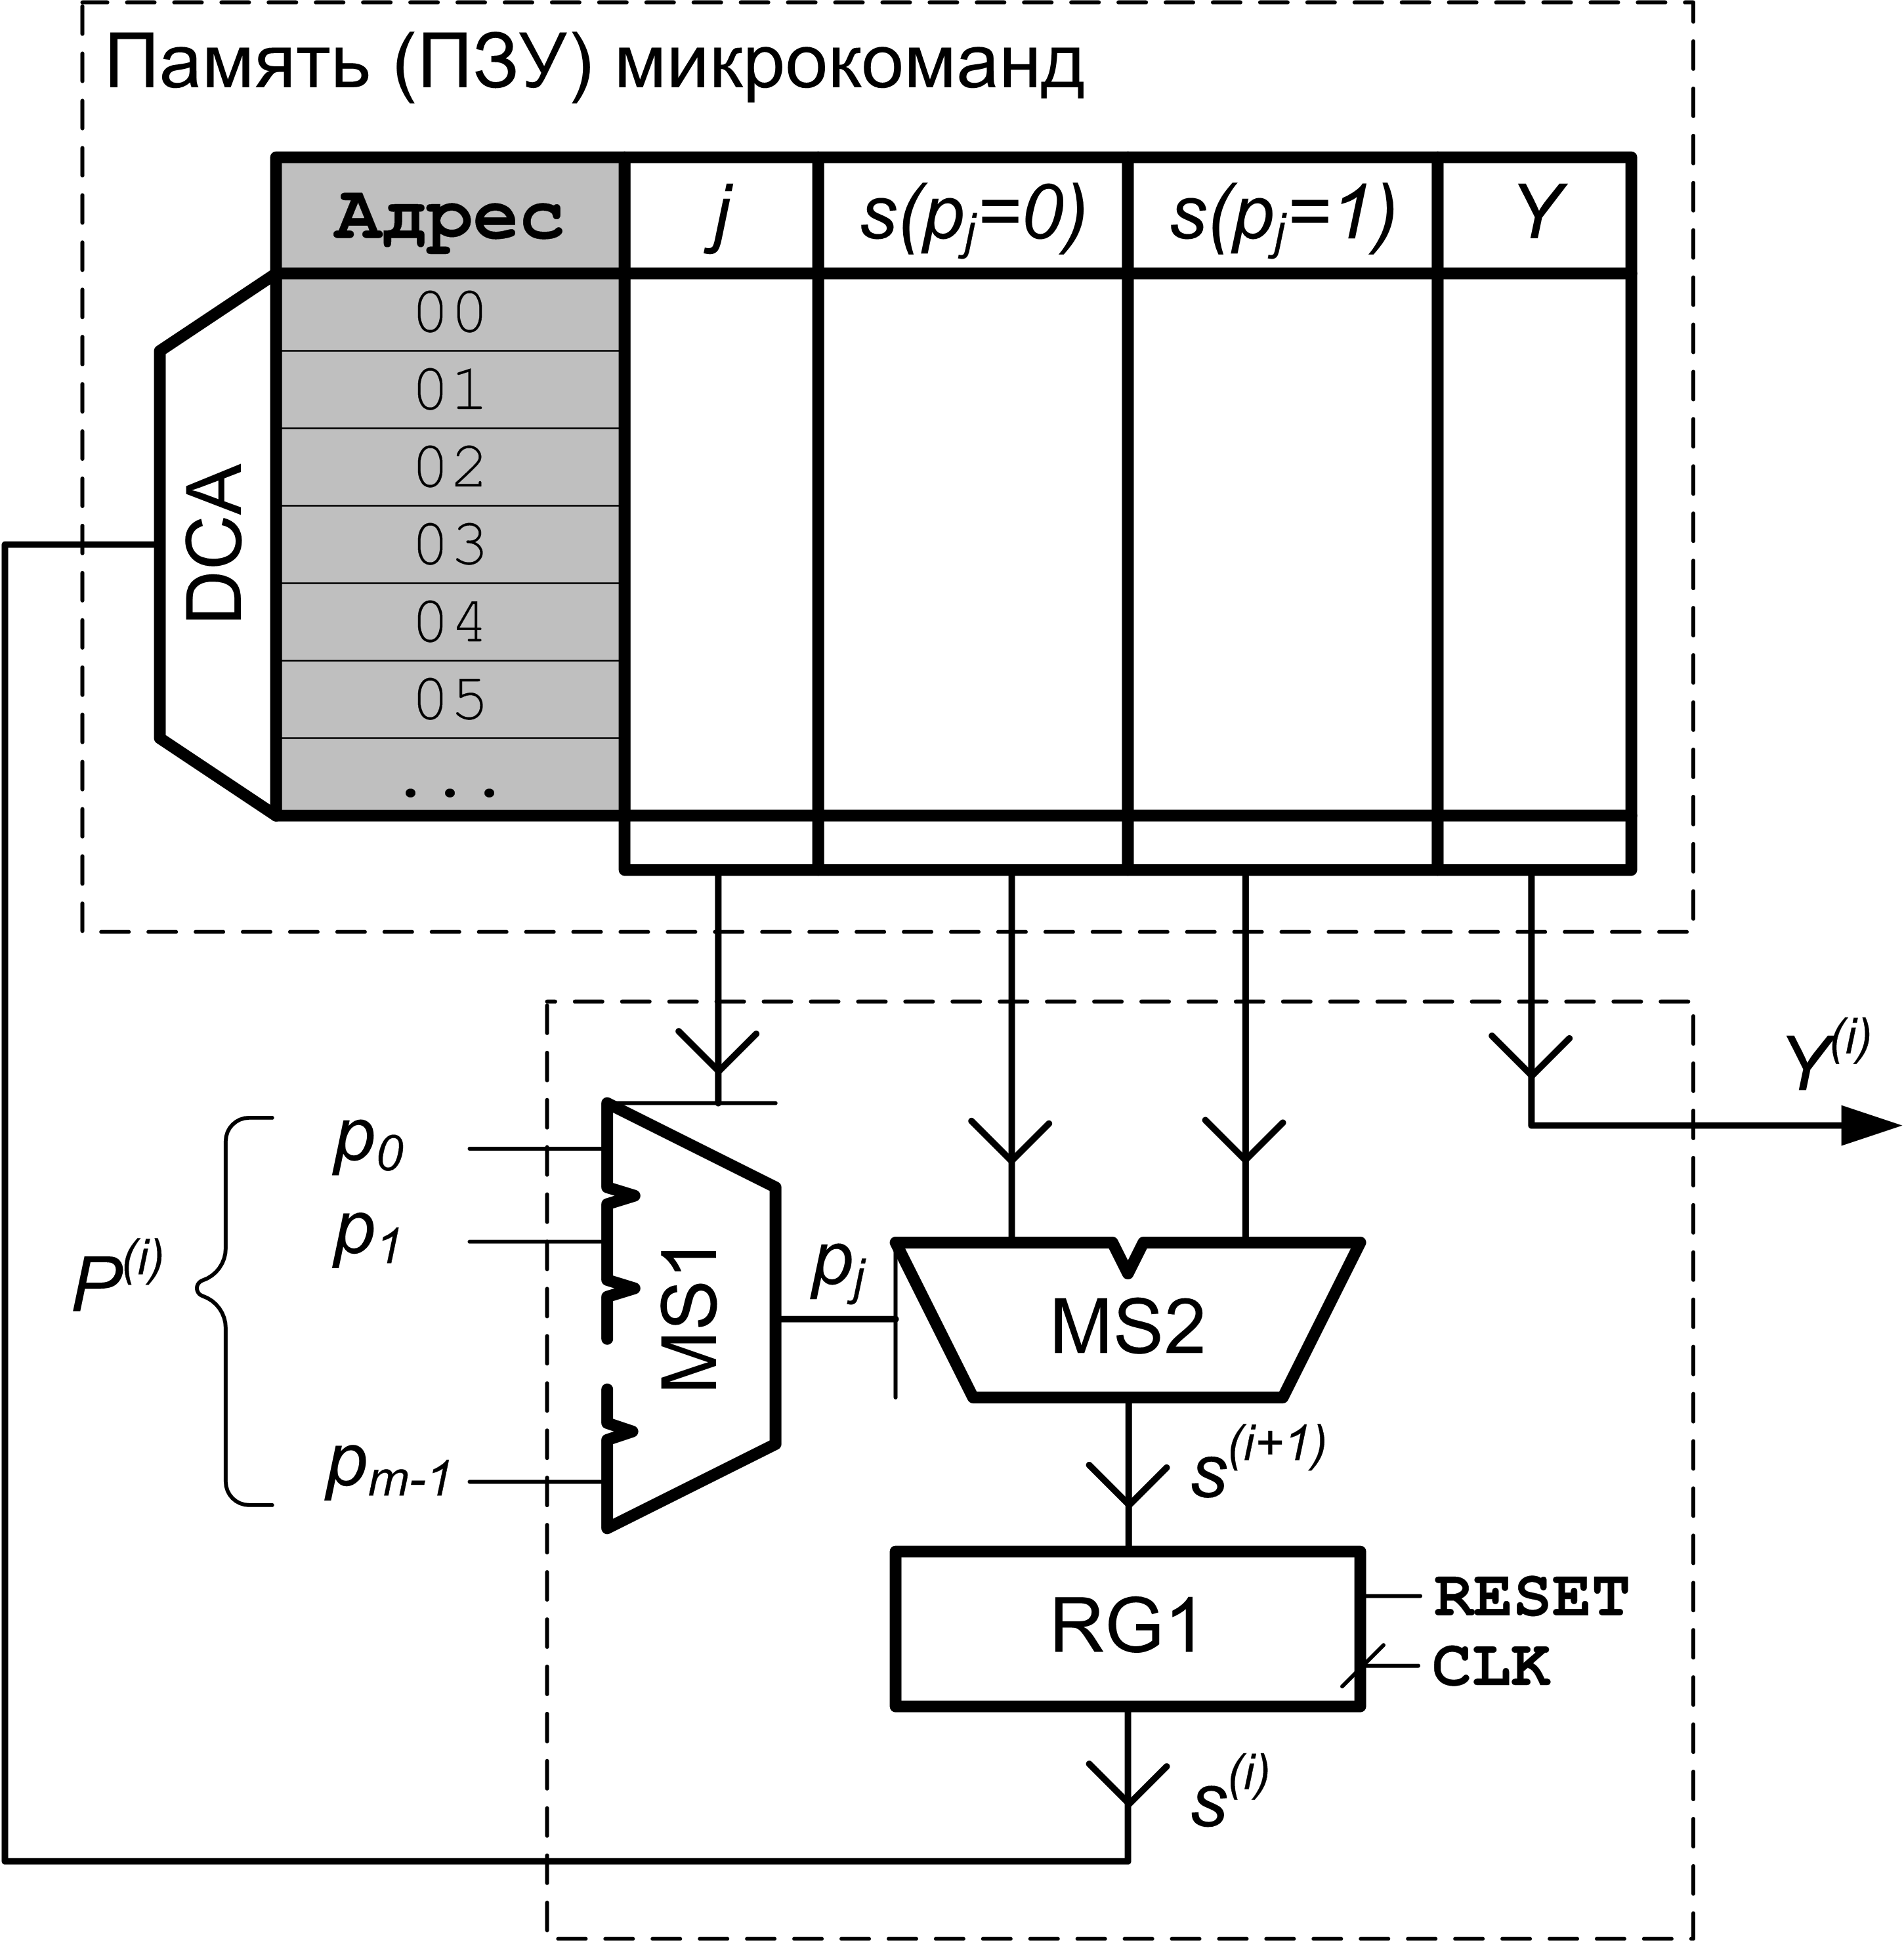
\includegraphics{fig/moore}
    \caption{Автомат Мура}
    \label{fig::ch::practice::Moore}
\end{figure}

В приведенных схемах микропрограммных автоматов выделены два блока --- <<Память (ПЗУ) микропрограмм>> и элементарное управляющее устройство. Текущему состоянию автомата $S^{(i)}$ соответствует адрес в памяти микропрограмм, то есть текущее состояние определяет адрес микрокоманды. Адрес (состояние) в течение такта снимается с выхода \Machine{RG1}. По завершению такта, в регистре \Machine{RG1} будет запомнено новое состояние, которое будет выдаваться в течение следующего такта. \Machine{RG1} переключается в каждом такте под управлением тактового сигнала \Machine{CLC}.

Ячейка памяти имеет для обоих автоматов общие части: 
\begin{itemize}
    \item поле $j$ --- выбор осведомительного сигнала (т.е. на управление \Machine{MS2} будет поступать значение осведомителного сигнала $p_j$);
    
    \item поле $S(p_j=0)$ --- новое состояние автомата, которое будет занесено в \Machine{RG1}, если $p_j=0$;
    
    \item поле $S(p_j=1)$ --- состояние, в которое перейдет автомат при $p_j=1$;    
\end{itemize}

Работа автомата начинается со сброса регистра \Machine{RG1} сигналом \texttt{RESET} в 0 --- автомат переходит в состояние $s_0$. 

Выход регистра \Machine{RG1} поступает на адресный вход памяти микрокоманд и через некоторое время значение ячейки памяти с указанным адресом поступает на выход модуля памяти. Значение поля $j$ управляет мультиплексором \Machine{MS1}, на выходе которого появляется значение осведомительного сигнала $p_j$, которое в свою очередь поступает на вход управления \Machine{MS2}. На выходе \Machine{MS2} появляется одно из двух состояний автомата: либо значение поля $S(p_j=0)$, либо --- поля $S(p_j=1)$. При переходе в следующий такт под управлением сигнала \Machine{CLC} регистр \Machine{RG1} запомнит новое состояние, сформировавшееся на выходе \Machine{MS2}.

В автомате Мили вектор управляющих сигналов снимается с выхода \Machine{MS2}, который осуществляет выбор из двух значений\footnote{
    На практике автомат Мили <<не прощает>> ошибок проектирования: когда значение сигнала $p_j$ меняется под воздействием управляющего сигнала в том же такте (такое бывает, когда значение $p_j$ снимается с выхода элемента логики, а не памяти, и соответсвенно может измениться в течение такта). Такое взаимовлияние может привести к <<гонкам>> осведомительных и управляющих сигналов и полной неопределенности в вопросе: <<в какое же из двух возможных состояний перейдет автомат Мили?>>
}, хранимых в памяти: $Y(p_j=0)$ и $Y(p_j=1)$;

В автомате Мура вектор управляющих сигналов определяется только текущим состоянием, поэтому снимается непосредственно с модуля памяти (поле $Y$).

В $i$-м такте работы управляющего устройства происходит следующее:
\begin{enumerate}
    \item Поступают осведомительные сигналы $P^{(i)}$. Эти осведомительные сигналы отражают изменения, произошедшие в предыдущем такте и в течение $i$-го такта не изменяются (так как снимаются обычно с выходов элементов памяти).
    
    \item Управляющее устройство формирует и выдает управляющие сигналы $i$-го такта. Также управляющее устройство определяет состояние $s^{(i+1)}$ в которое оно перейдет по завершении $i$-го такта. Значения управляющих сигналов стабилизируются, они распространяются по схеме и на сответствующих входях элементов памяти устанавливаются корректные значения.
    
    \item В конце такта (в зависимости от управляющих сигналов) в операционной части происходит защелкивание необходимых значений в элементах памяти. В частности, желательно сохранять в элементах памяти значения осведомительных сигналов.
\end{enumerate}

Одному такту работы схемы автомата Мили на рисунке \ref{fig::ch::practice::Mili} можно сопоставить фрагменты граф-схемы алгоритма, приведенные на рисунке \ref{fig::ch::practice::MiliAlg}. Состояния автомата выделены серыми кружками-пометками. Автомат Мили в том же такте реагирует (управляющими сигналами) на осведомительные сигналы.

\begin{figure}[!ht]
    \centering
    \begin{tabular}{c|c}
        \raisebox{-.5\height}{
            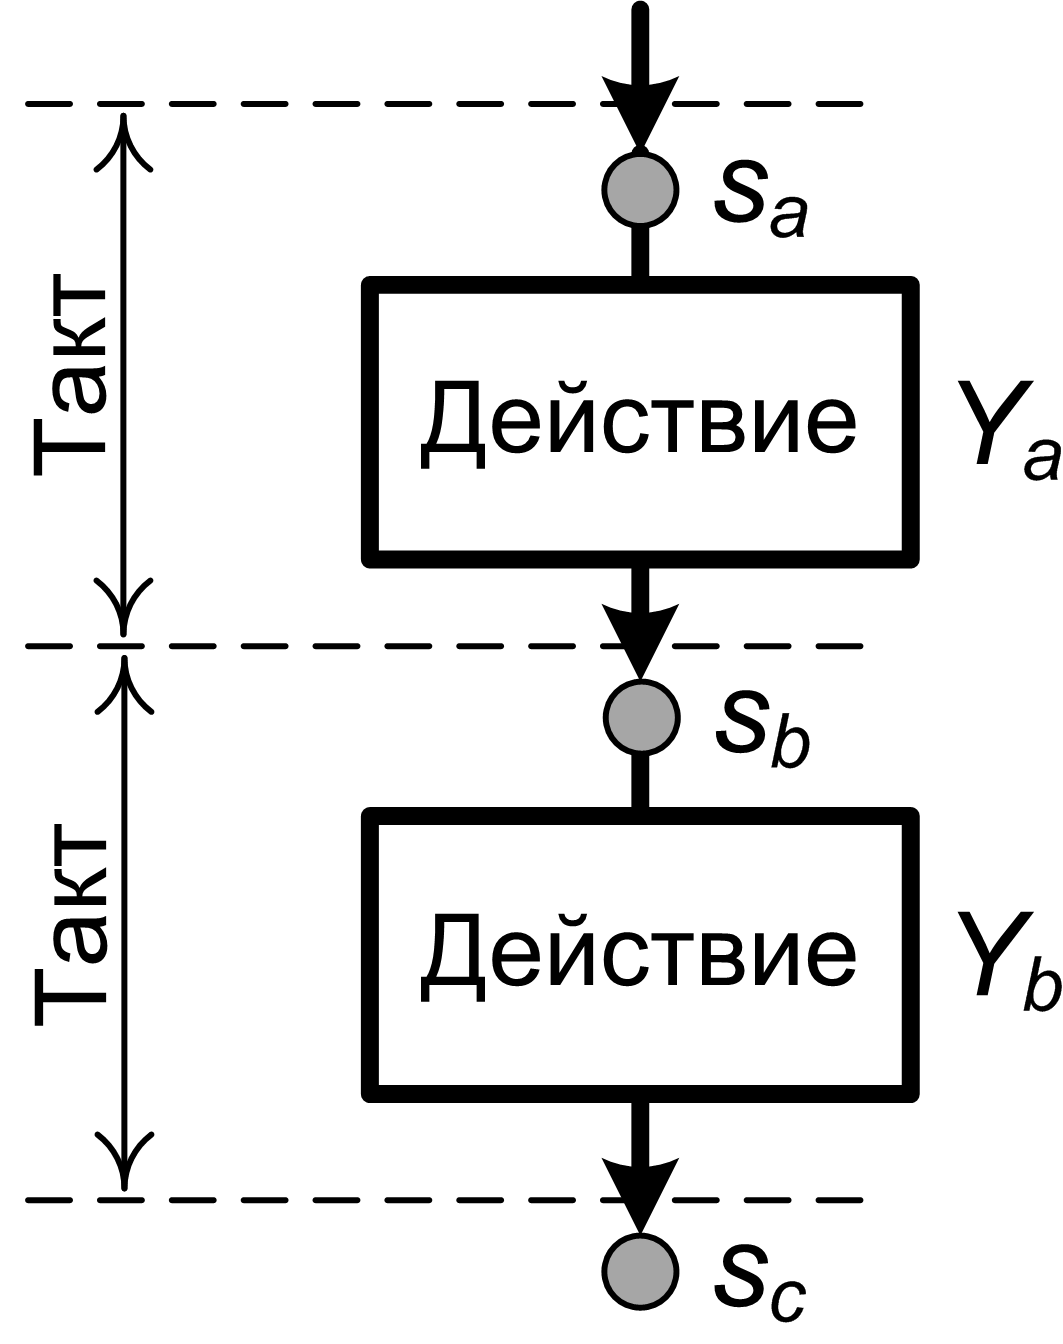
\includegraphics{fig/MiliAlgSeq}
        }
        &
			\raisebox{-.5\height}{
				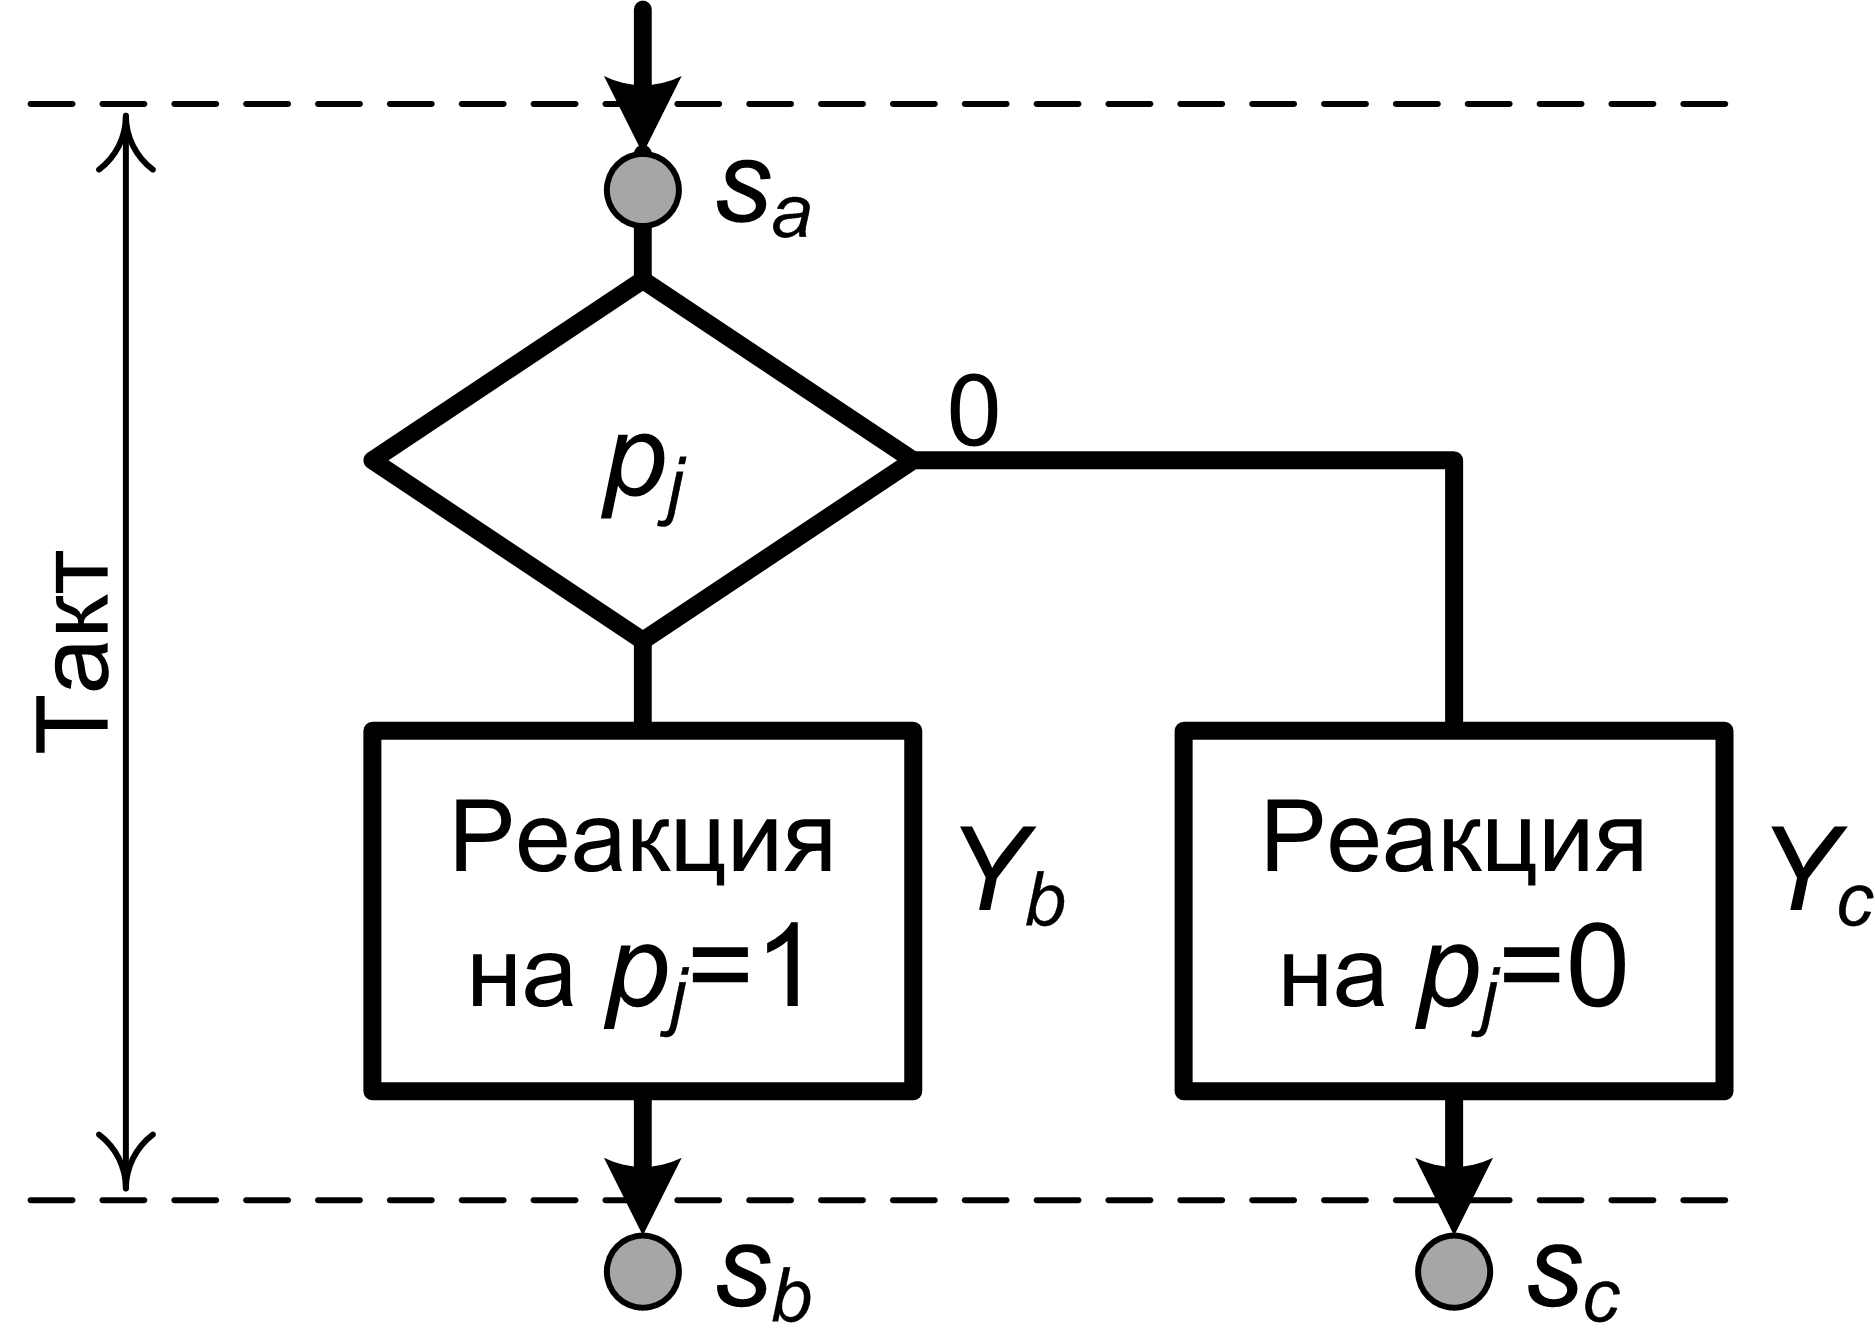
\includegraphics{fig/MiliAlgIf}
			} 
			\\
        {\xymatrix{
            S_a \ar@{->}[r]^{*|Y_a} 
                &S_b \ar@{->}[r]^{*|Y_b} 
					&S_c 
        }}
		&
			{\xymatrix{
				S_a \ar@{->}@/^/[r]^{\bar{p}_j|Y_c} 
					\ar@{->}@/_/[dr]_{p_j|Y_b} 
					&S_c \\
				*{} &S_b
			}}
			\\
    \end{tabular}
    \caption{Примеры фрагментов алгоритмов, реализуемых автоматом Мили за один такт}
    \label{fig::ch::practice::MiliAlg}
\end{figure}

Граф-схема, соответствующая такту работы автомата Мура (рис. \ref{fig::ch::practice::Moore}) приведена на рисунке \ref{fig::ch::practice::MooreAlg}. Автомат Мура реагирует на осведомительные сигналы только в следующем такте. 

\begin{figure}[!ht]
    \centering
    \begin{tabular}{c|c}
        \raisebox{-.5\height}{
            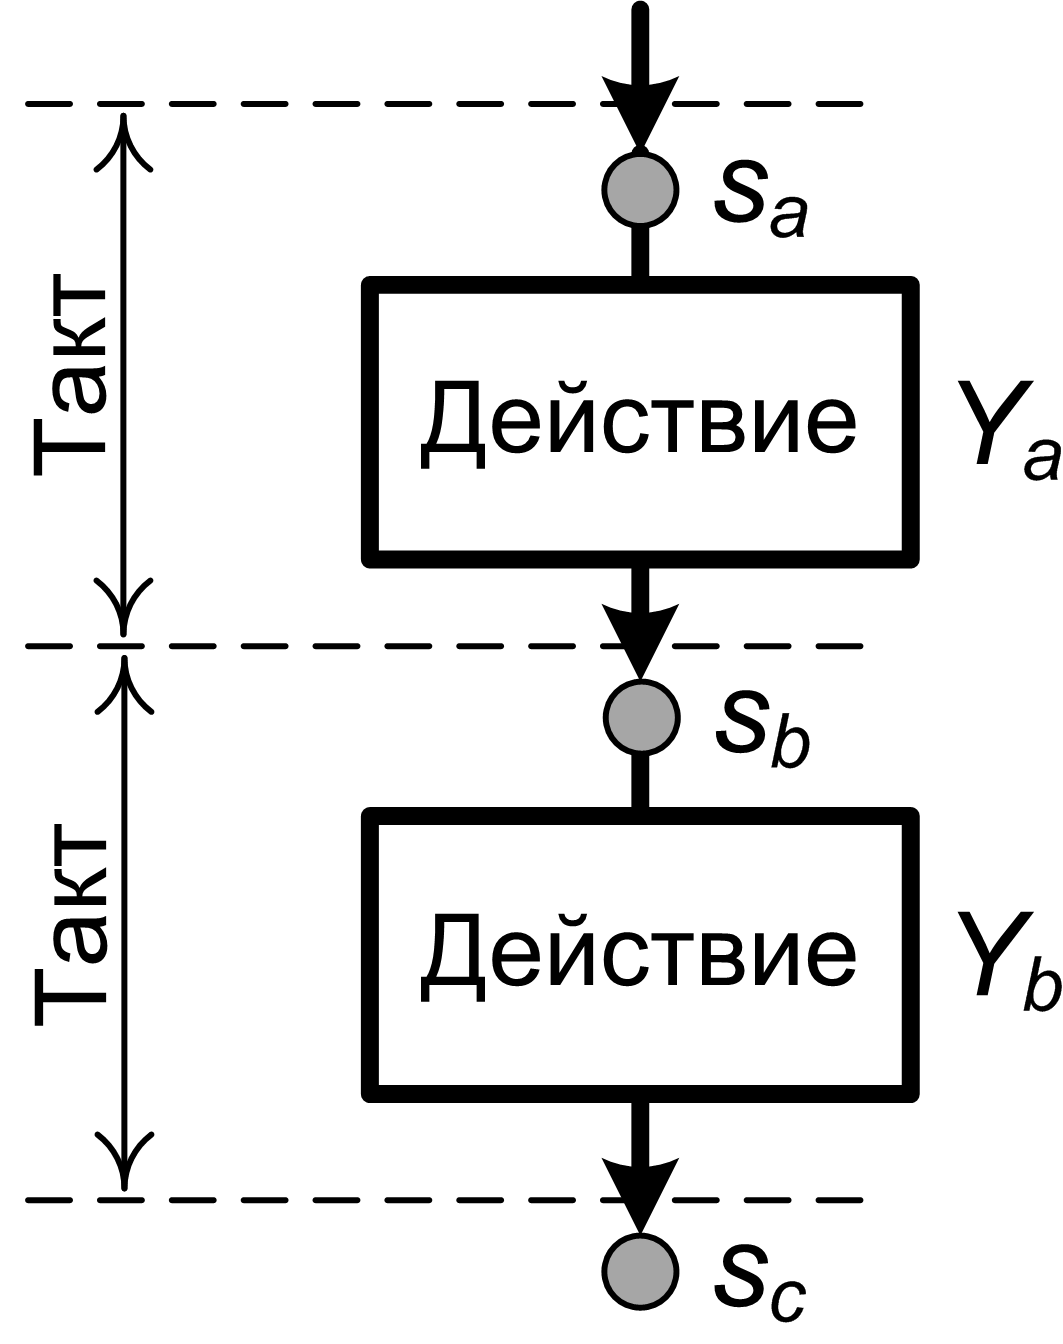
\includegraphics{fig/MooreAlgSeq}
        }
        &
			\raisebox{-.5\height}{
                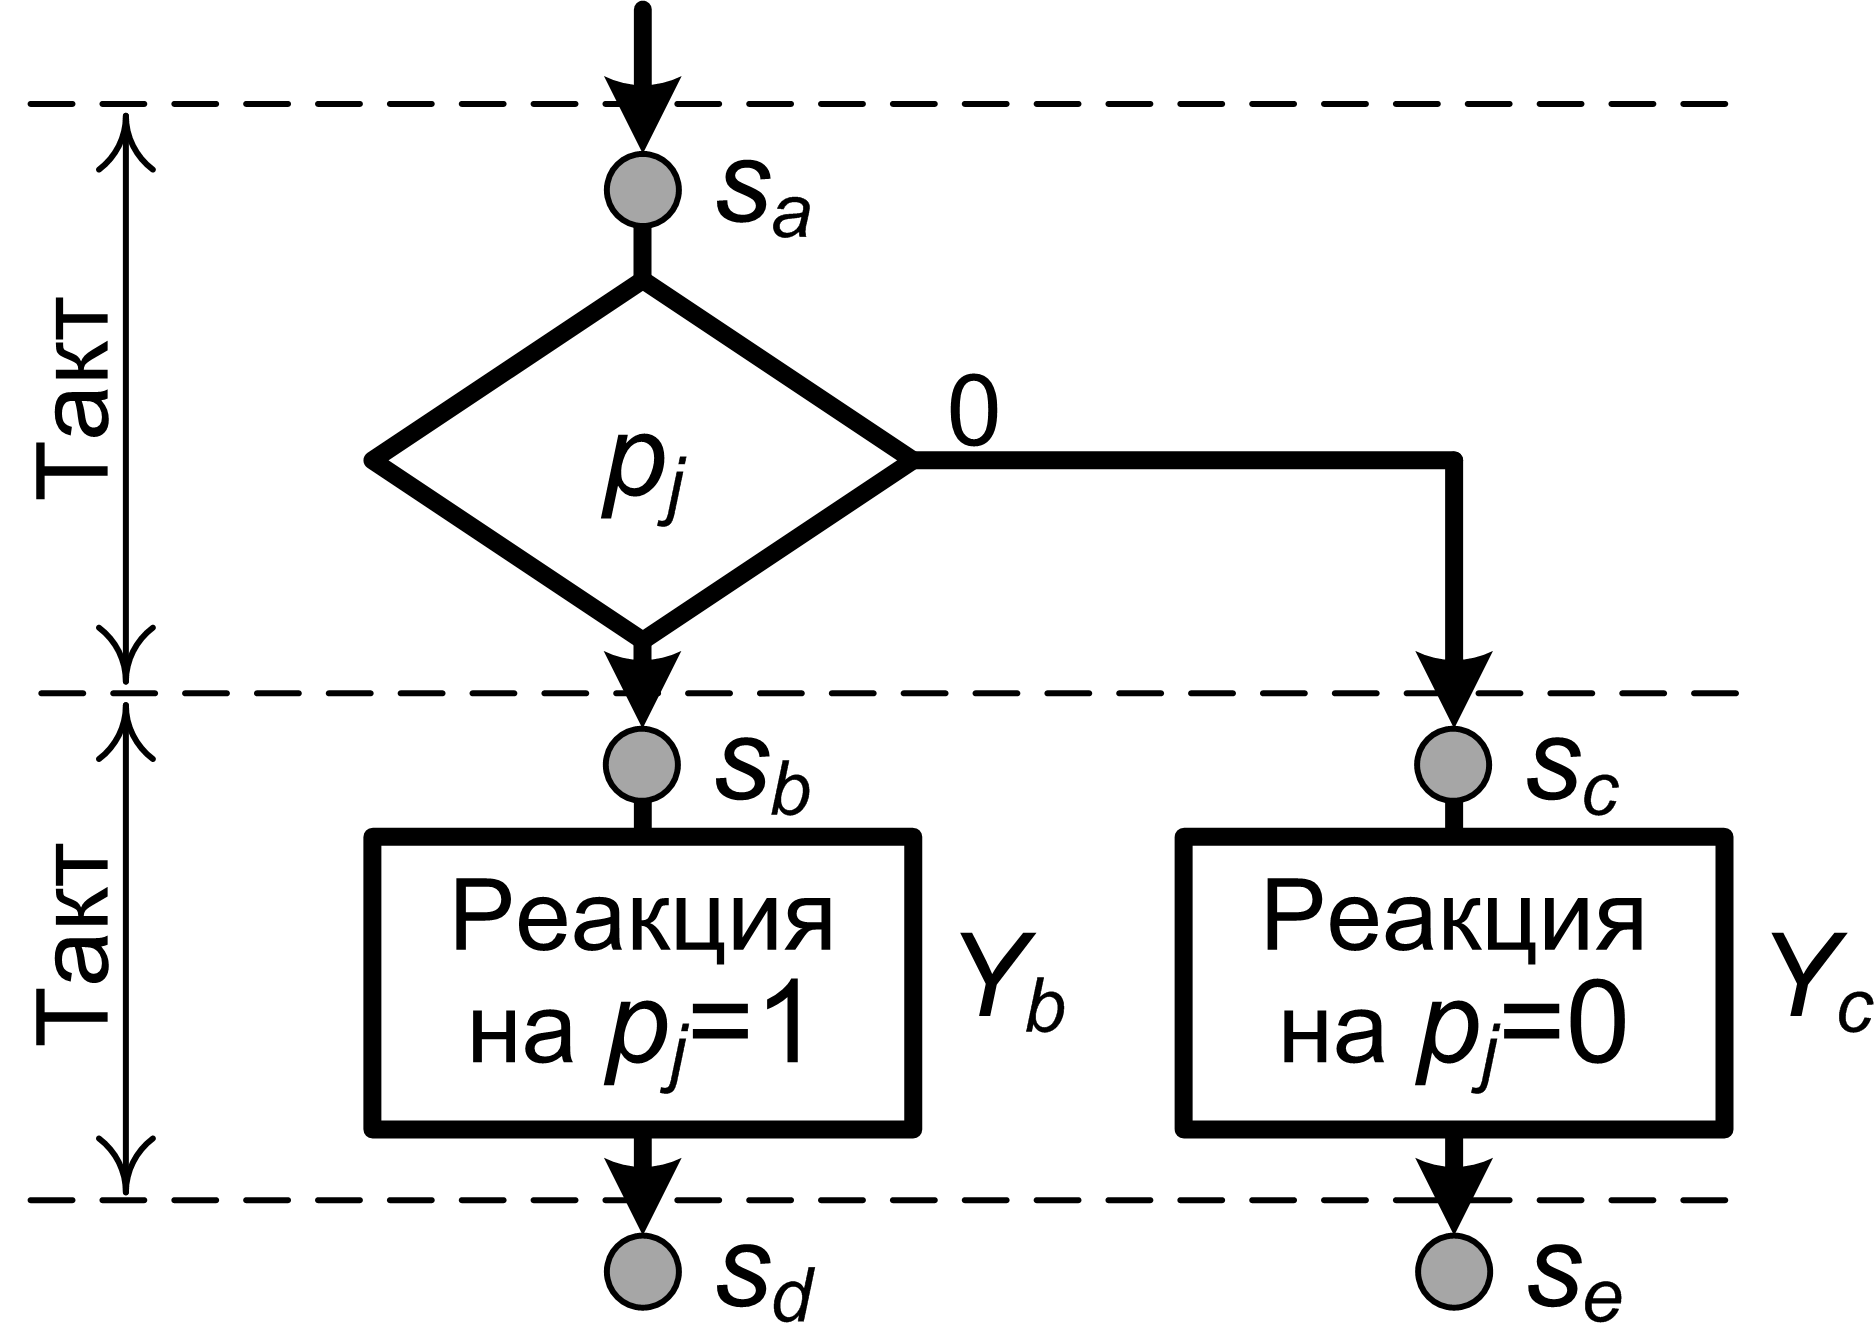
\includegraphics{fig/MooreAlgIf}
            }
			\\
        {\xymatrix{
            S_a|Y_a \ar@{->}[r]^{*} 
                &S_b|Y_b \ar@{->}[r]^{*} 
                    &S_c| \\
        }}
        &
            {\xymatrix{
                S_a|\Machine{0h} \ar@{->}@/^/[r]^{\bar{p}_j} 
                    \ar@{->}@/_/[dr]_{p_j} 
                    &S_c|Y_c \ar@{->}[r]^{*} 
                        &S_e|
                        \\
                *{} 
                    &S_b|Y_b \ar@{->}[r]^{*} 
                        &S_d|
            }}            
    \end{tabular}
    \caption{Примеры фрагментов алгоритма, реализуемых автоматом Мура за один такт}
    \label{fig::ch::practice::MooreAlg}
\end{figure}

Видно, что автомат Мура тратит отдельный такт на анализ осведомительного сигнала, при этом в таком такте, конечно могут выдаваться и управляющие сигналы (в приведенном примере на Рис. \ref{fig::ch::practice::MooreAlg} выдается \Machine{0h}). То есть, можно совместить вершину процесса и условную вершину в одном состоянии, если процесс на условие не влияет и тогда процесс и анализ условия \emph{совмещаются} во времени. В противном случае, если имелось в виду, что \emph{после} определенных действий, следует проанализировать осведомительный сигнал, то следует выделить два состояния (см. пример на рисунке \ref{fig::ch::practice::MooreAlgFictive}).
\begin{figure}[!ht]
    \centering
    \begin{tabular}{c|c}
        \raisebox{-.5\height}{
            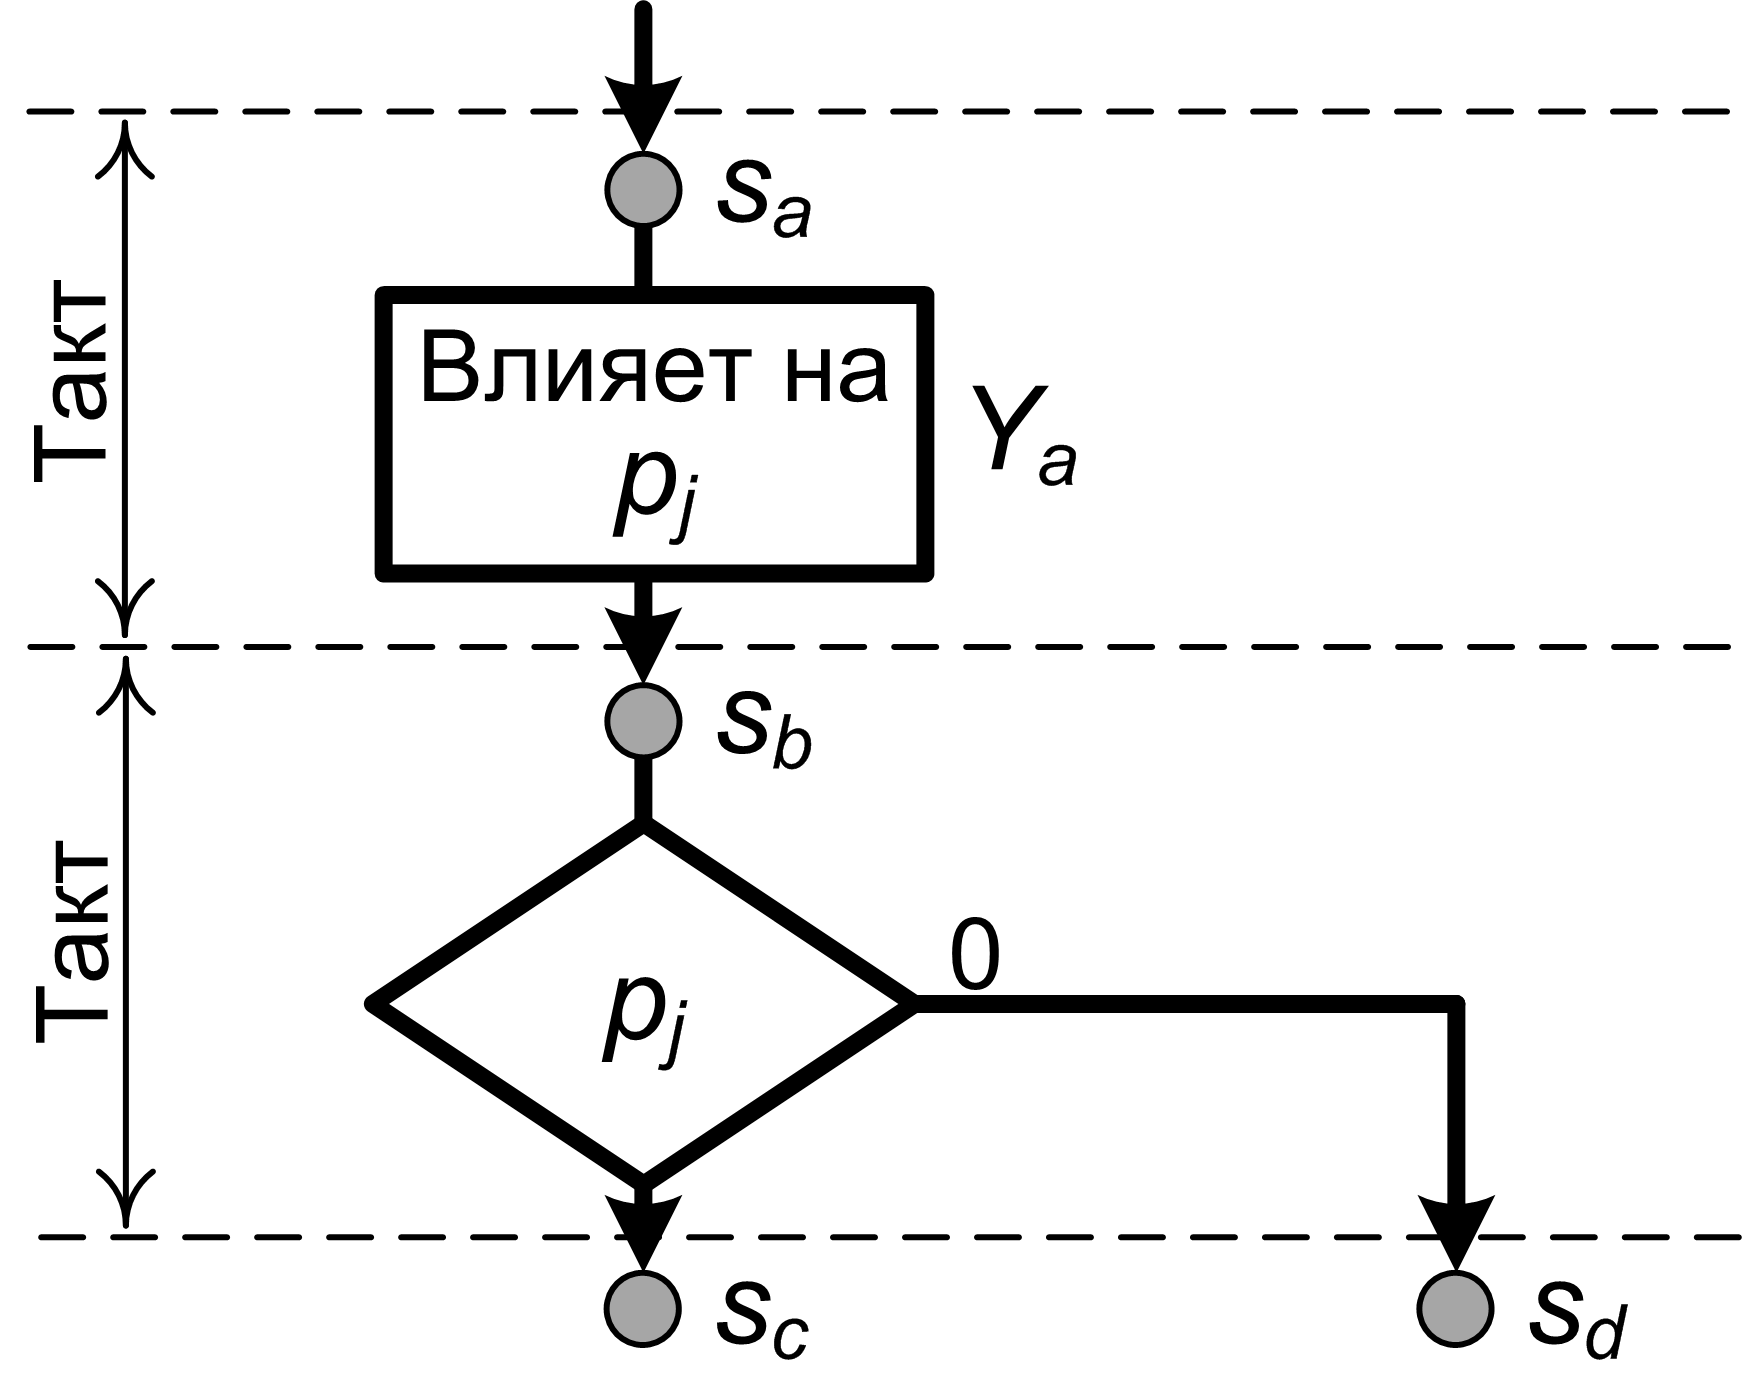
\includegraphics{fig/MooreIfTwo}
        }
        &
			\raisebox{-.5\height}{
                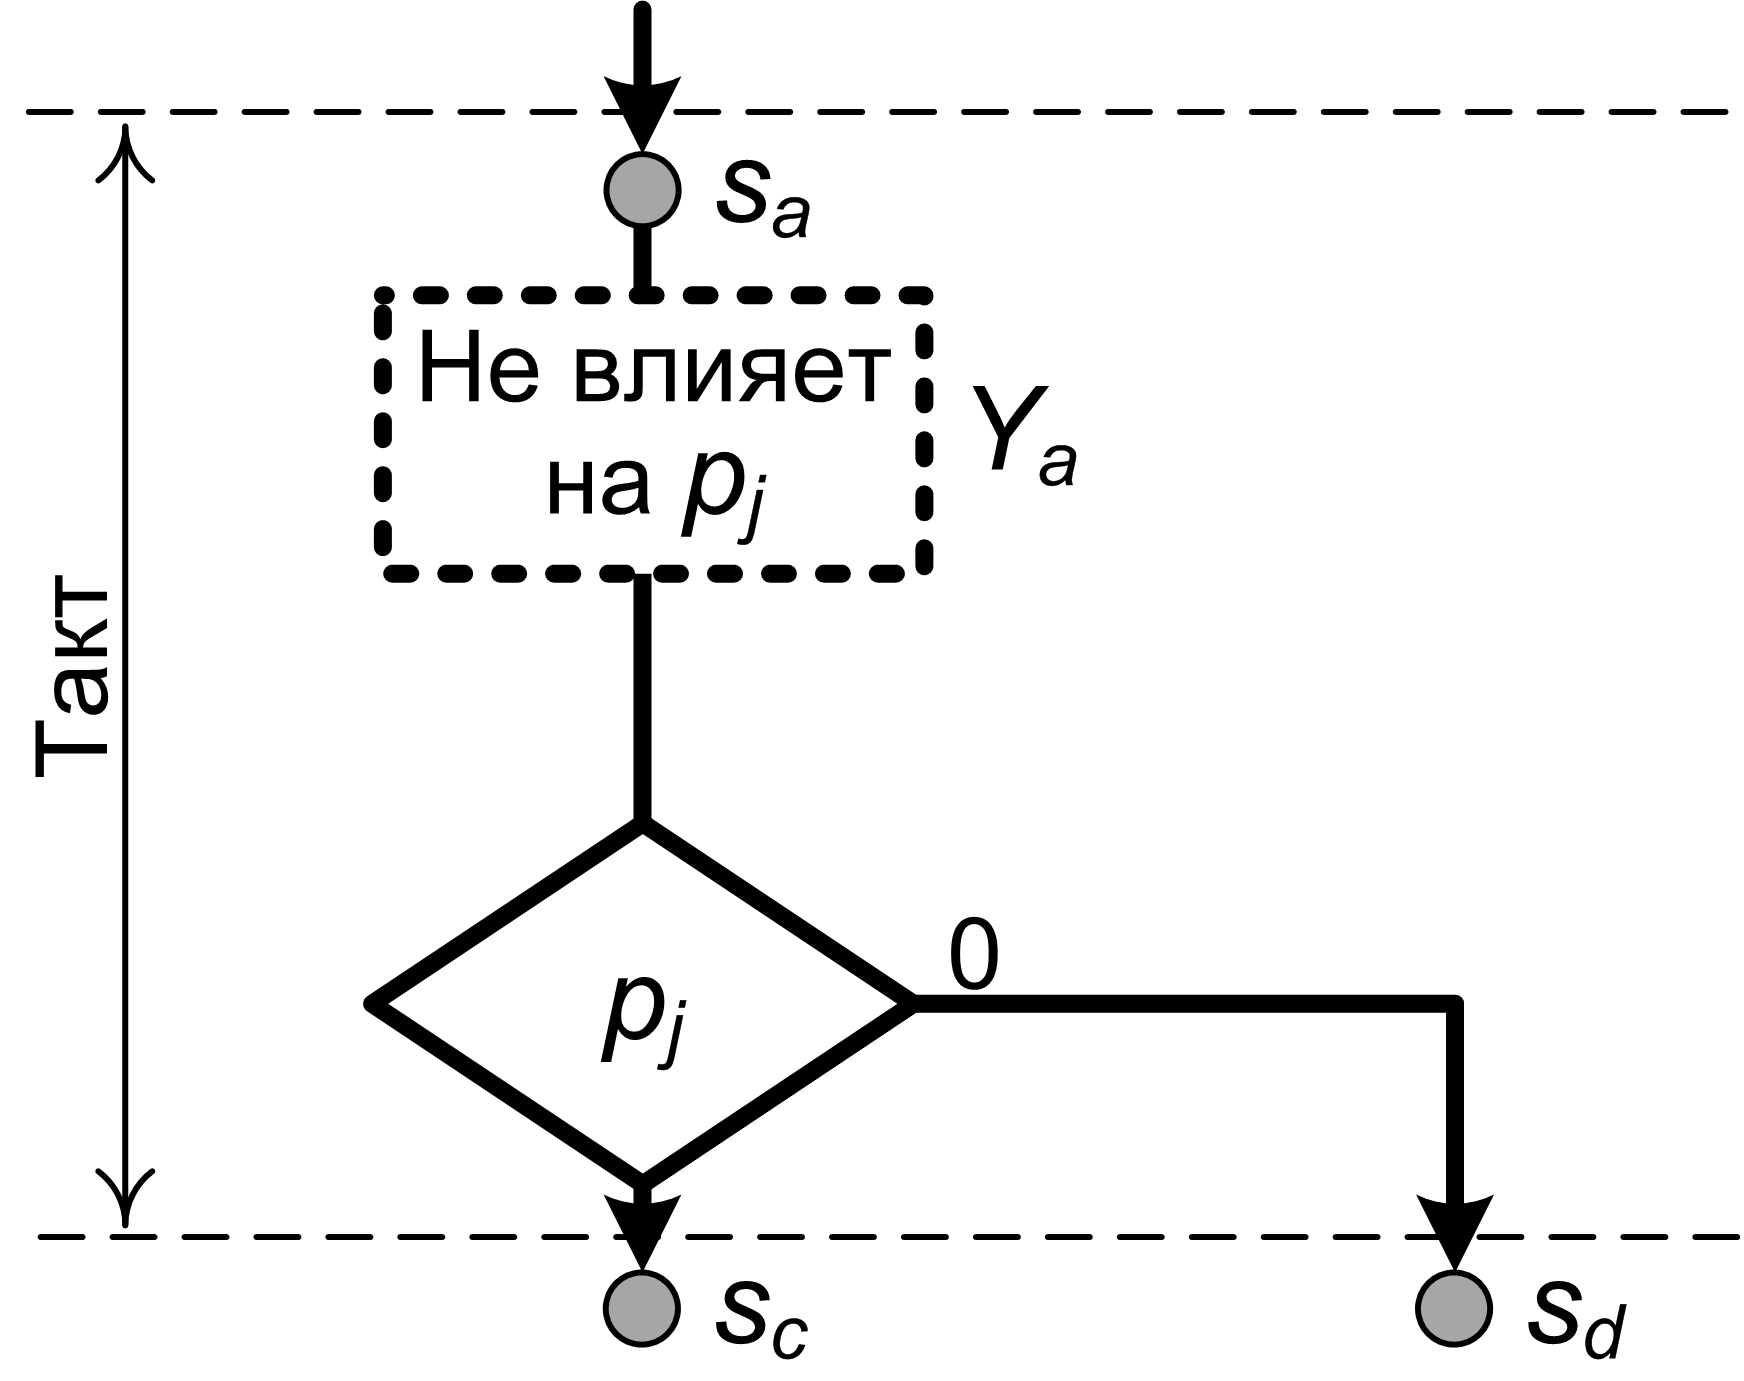
\includegraphics{fig/MooreIfOne}
            }
			\\
        {\xymatrix{
            S_a|Y_a \ar@{->}[r]_{*} 
                &S_b|\Machine{0h} \ar@{->}@/^/[r]^{\bar{p}_j}  
                                  \ar@{->}@/_/[dr]_{p_j} 
                    &S_d|
                    \\
            *{} 
                &*{}
                    &S_c|
        }}            
        &
            {\xymatrix{
                S_a|Y_a \ar@{->}@/^/[r]^{\bar{p}_j}  
                                      \ar@{->}@/_/[dr]_{p_j} 
                    &S_d|
                    \\
                *{}
                    &S_c|
        }}            
    \end{tabular}
    \caption{Особенности выделения состояний автомата Мура}
    \label{fig::ch::practice::MooreAlgFictive}
\end{figure}


На указанные фрагменты можно разбить любую произвольную схему алгоритма. Также при составлении алгоритма следует учитывать указанные особенности автомата, выполняющего этот алгоритм. Детальное обсуждение особенностей находится за рамками данного курса, поэтому далее рассматривается пример микропрограммирования, который позволить понять суть микропрограммного управления.

\subsection{Соглашения о взаимодействии с ЦУУ}

Особенности взамодействия ОЧ множительного устройства и ЦУУ были изложены в самом начале раздела \ref{ch::practice}. Введем следующие обозначения сигналов:
\begin{itemize}
    \item $p_0\Machine{(TASK)}$ --- <<Задание на шине>> от ЦУУ;
    \item $p_1\Machine{(BUS)}$ --- <<Шина твоя>> от ЦУУ;
    \item $y_0\Machine{(READY)}$ --- <<Свободен>> в ЦУУ;
    \item $y_1\Machine{(RESULT)}$ --- <<Результат готов>> в ЦУУ;
    \item \Machine{CLK} --- тактовые импульсы, синхронизирующие все устройства вычислительной системы в целом;
    \item \Machine{X(DATA)} --- данные на шине данных, могут выдаваться как ЦУУ (исходные операнды), так и множительным устройством (результат).
\end{itemize}

Изменение сигналов принято изображать на временной диаграмме. Высокий уровень сигнала на диаграмме соответствует логической единице, низкий --- нулю.

\begin{figure}[!ht]
    \centering
    \includegraphics{fig/timings.1}
    \caption{Временная диаграмма получения задания}
    \label{fig::ch::practice::timingsTr}
\end{figure}

Состояние шины (жгута) изображается по особому: так как на диаграмме обычно нет места, чтобы изобразить все линии шины по отдельности, то состояние шины изображают как один сигнал (см. сигнал \Machine{X(DATA)}). Когда состояние шины не имеет значения (на рисунке \ref{fig::ch::practice::timingsTr} это такты 0 и 3), то рисуют линию посередине между высоким и низким уровнем. При этом по шине могут передаваться данные для других устройств.

Когда на шину поступают данные, которые важны, их изображают двумя линиями, проведенными на высоком и низком уровнях одновременно (такты 1, 2 на рисунке \ref{fig::ch::practice::timingsTr}), а если нужно указать значение двоичного вектора на шине, то между линиями пишут соответствующее шестнадцатиричное значение.

На рисунке \ref{fig::ch::practice::timingsTr} изображена временная диаграмма получения задания от ЦУУ. Устройства следуют следующим соглашениям.
\begin{enumerate}
    \item УЧ выдает в ЦУУ сигнал $y_0\Machine{(READY)}$. См. такт 1. Таким образом УЧ сообщает ЦУУ, что множительное устройство готово решать новую задачу. Сигнал будет удерживаться до тех пор, пока ЦУУ не даст задание. 
    
    \item Когда ЦУУ потребуется выполнить умножение, то оно, убедившись, что множительное устройство готово ($y_0=1$), выдает в УЧ сигнал $p_0\Machine{(TASK)}$. См. такт 3. В последующих тактах ЦУУ будет выдавать фрагменты задания $\Machine{D}_1,\ldots,\Machine{D}_n$. В общем случае, задание состоит из одного фрагмента.
    
    ЦУУ выдает сигнал $p_0\Machine{(TASK)}$ только в течение одного такта.
    
    \item УЧ \emph{должна} в следующем такте, после получения сигнала  $p_0\Machine{(TASK)}$ от ЦУУ снять сигнал $y_0\Machine{(READY)}$ и начать чтение с шины первого фрагмента задания. См. такт 4. Пока УЧ решает задачу, сигнал $y_0\Machine{(READY)}$ не должен выдаваться.
\end{enumerate}

На рисунке \ref{fig::ch::practice::timingsRr} изображена временная диаграмма выдачи результата в ЦУУ. 

\begin{figure}[!ht]
    \centering
    \includegraphics{fig/timings.2}
    \caption{Временная диаграмма выдачи результата}
    \label{fig::ch::practice::timingsRr}
\end{figure}

\begin{enumerate} 
    \item УЧ выдает в ЦУУ сигнал $y_1\Machine{(RESULT)}$. См. такт 1. УЧ будет ждать момента, когда ЦУУ освободит шину и будет удерживать этот сигнал, пока не получит разрешение на передачу. См. такты 1-3. Количество тактов, в течение которых ЦУУ освобождает шину, варьируется, и непоправимой ошибкой будет выдача результата на <<занятую>> шину.

    \item ЦУУ, убедившись, что результат готов, выдает в течение одного такта сигнал $p_1\Machine{(BUS)}$. См. такт 3.
    
    \item УЧ, приняв сигнал $p_1\Machine{(BUS)}$ в следующем такте \emph{должно} снять сигнал $y_1\Machine{(RESULT)}$ и начать выдавать первый фрагмент результата. См. такт 4.
    
    \item УЧ как можно раньше должно выдать в ЦУУ сигнал $y_0\Machine{(READY)}$. Обычно, сигнал $y_0\Machine{(READY)}$ выдается в том же такте, в котором выдается последний фрагмент результата. См. такт $(n+3)$.
\end{enumerate}


\subsection{Пример микропрограммирования}
\label{ss::ch::practice::software::example}

В качестве примера рассматривается задача получения дополнительного кода из прямого. Несомненно, эту задачу можно решить проще.

Операционная часть устройства приведена на рисунке \ref{fig::ch::practice::dcconverter}.

\begin{figure}[!ht]
    \centering
    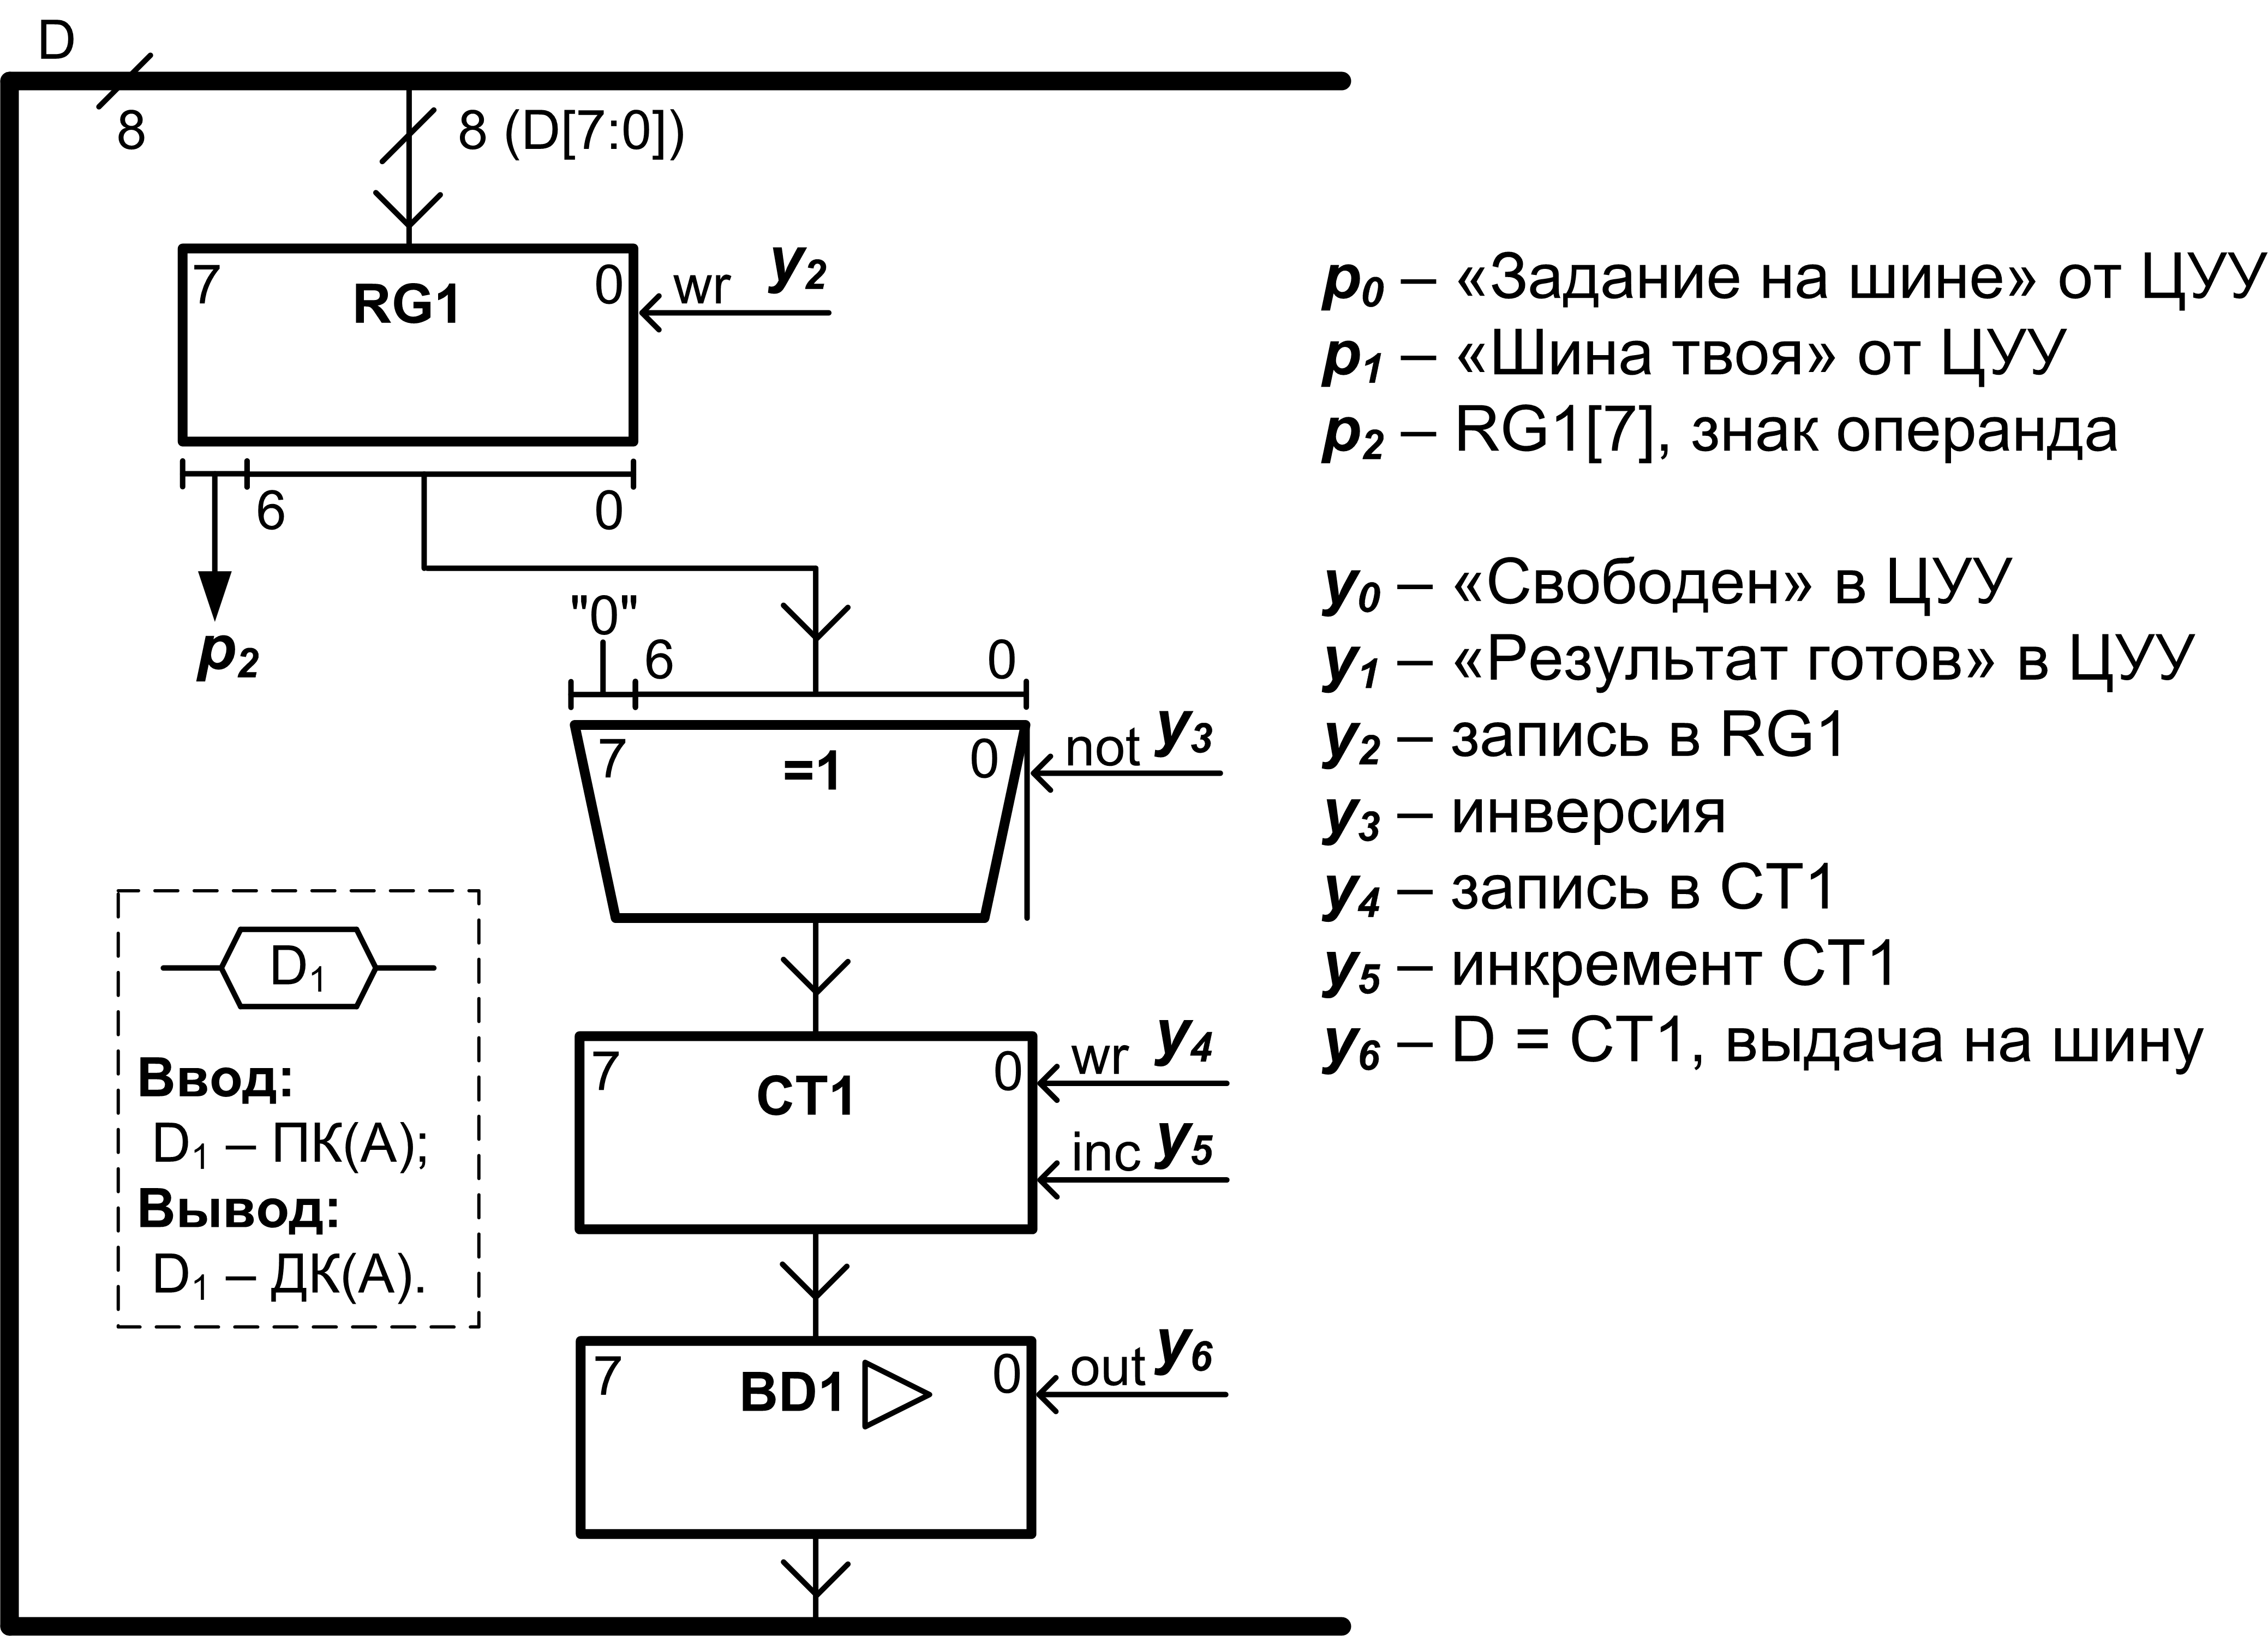
\includegraphics{fig/dcconverter}
    \caption{Операционная часть преобразователя $\Machine{ПК}\mapsto\Machine{ДК}$}
    \label{fig::ch::practice::dcconverter}
\end{figure}

Назначение осведомительных и управляющих сигналов следующее:
\begin{itemize}
    \item $p_0\Machine{(TASK)}$ --- <<Задание на шине>> от ЦУУ;
    \item $p_1\Machine{(BUS)}$ --- <<Шина твоя>> от ЦУУ;
    \item $y_0\Machine{(READY)}$ --- <<Свободен>> в ЦУУ;
    \item $y_1\Machine{(RESULT)}$  --- <<Результат готов>> в ЦУУ;
    
    \item $p_2$ --- \Machine{RG1[7]}, знак операнда;
    \item $y_2$ --- запись в \Machine{RG1}
    \item $y_3$ --- инверсия;
    \item $y_4$ --- запись в \Machine{CT1};
    \item $y_5$ --- инкремент \Machine{CT1};
    \item $y_6$ --- \Machine{X=CT1}, выдача результата на шину.
\end{itemize}

С помощью данной операционной части задачу можно решить так:
\begin{enumerate}
    \item получить задание и записать операнд в \Machine{RG1} ($y_2$); 
    \item если знак операнда $p_2=0$, то перейти к шагу \ref{en:ch::practice::dcconverter:positive}, иначе к шагу \ref{en:ch::practice::dcconverter:negative};
    \item \label{en:ch::practice::dcconverter:positive} записать модуль операнда в \Machine{CT1} ($y_4$); перейти к шагу \ref{en:ch::practice::dcconverter:end};
    \item \label{en:ch::practice::dcconverter:negative} записать инвертированный модуль операнда в \Machine{CT1} ($y_3,y_4$);
    \item инкрементировать \Machine{CT1} ($y_5$);
    \item \label{en:ch::practice::dcconverter:end} в \Machine{CT1} получен результат; выдать его в ЦУУ.
\end{enumerate}

В зависимости от управляющего автомата, в этот базовый алгоритм придется внести некоторые изменения. В следующих параграфах приводятся микропрограммные реализации данного алгоритма\footnote{Следует отметить, что приведенные реализации, как для автомата Мили, так и Мура, можно оптимизировать. Оптимизация не была сделана авторами с целью упростить изложение} с помощью автоматов Мили и Мура.


\subsubsection{Автомат Мили}

На рисунке \ref{fig::ch::practice::miliPcDcAlgo} изображен алгоритм\footnote{Строго говоря, это метод, а не алгоритм --- алгоритм обязан завершаться через конечное число шагов \cite{bib:knuth:artOfProgramming1}} работы преобразователя $\Machine{ПК}\mapsto\Machine{ДК}$ под управлением автомата Мили. Серыми кружками отмечаются состояния ($s_0$--$s_5$). 

\begin{figure}[!ht]
    \centering
    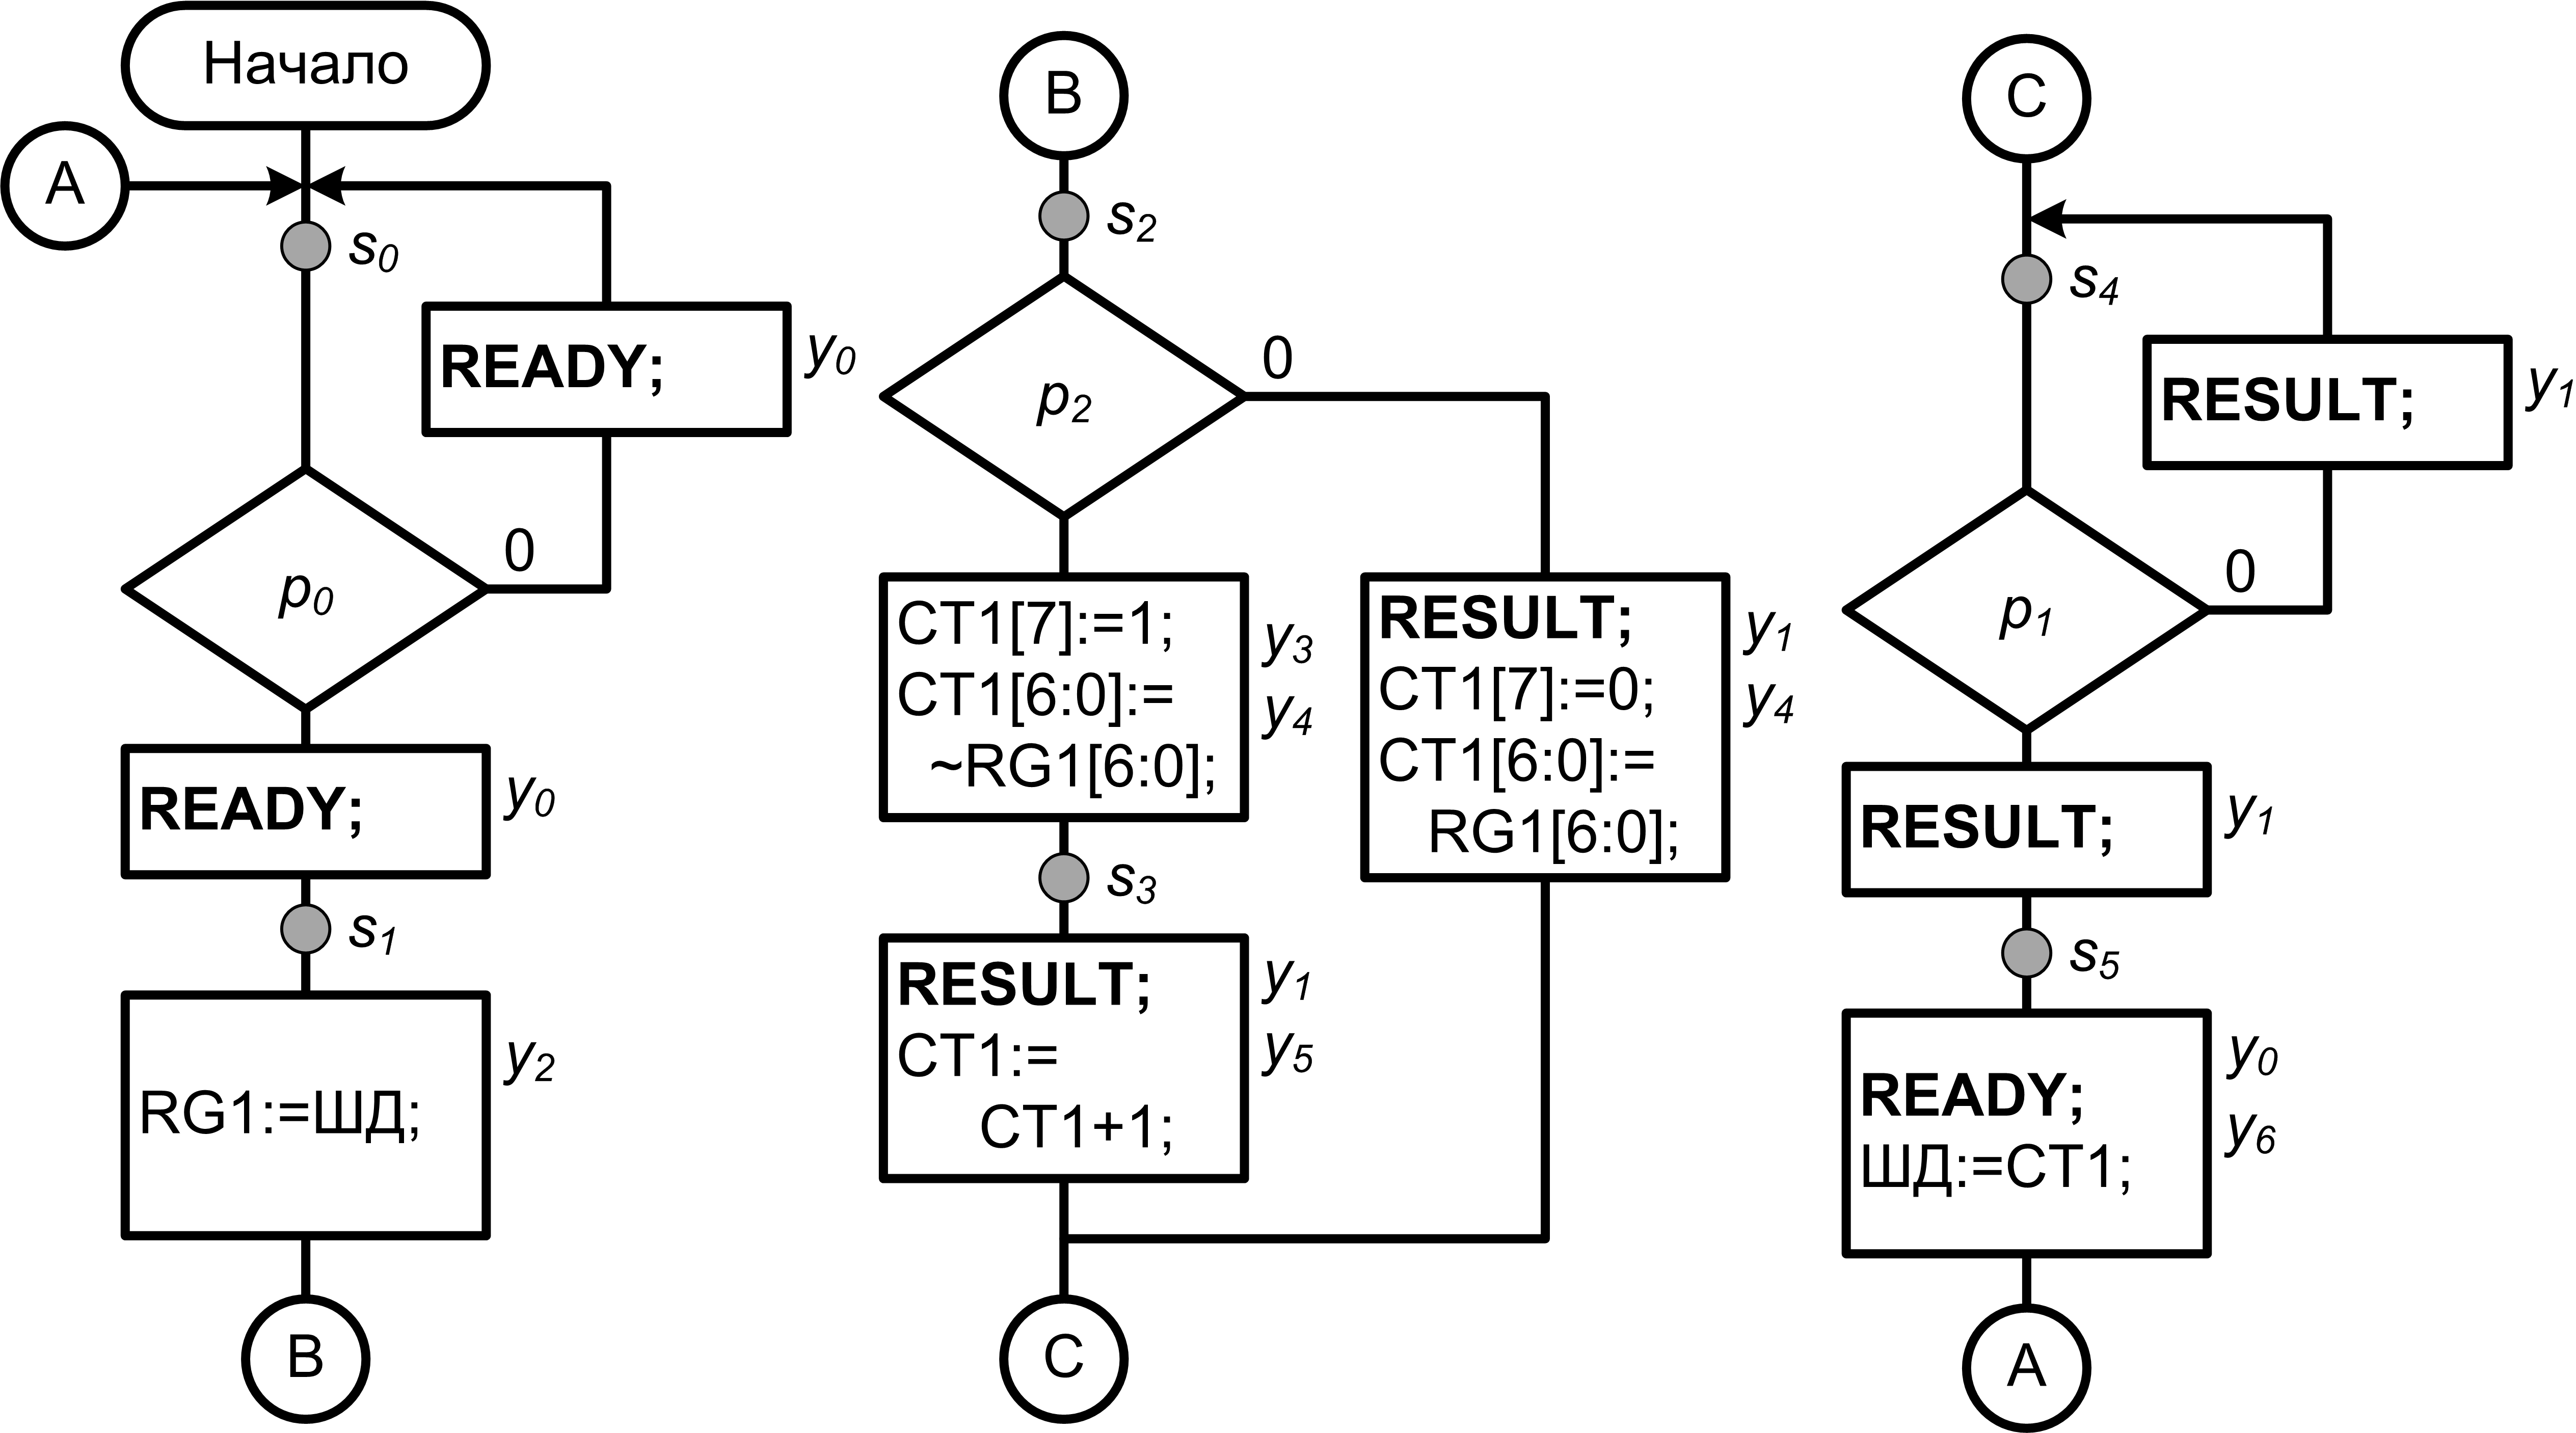
\includegraphics[width=\textwidth]{fig/miliPcDcAlgo}
    \caption{Алгоритм работы преобразователя $\Machine{ПК}\mapsto\Machine{ДК}$ под управлением автомата Мили}
    \label{fig::ch::practice::miliPcDcAlgo}
\end{figure}

Отметка состояния ставится над условной вершиной (см. рисунок \ref{fig::ch::practice::MiliAlg}). При отсутствии таковой, например, между двумя последовательными блоками процеса\footnote{Блок процесса обозначается на блок-схеме прямоугольником}, вводится фиктивная вершина условия с одинаковым исходом для истины и лжи. В данном примере фиктивные условные вершины введены для состояний $s_1$, $s_3$, $s_5$.

Также следует отметить, что сигнал $y_0\Machine{(ACK)}$ (<<Задание принял>>) выдается в следующем такте (при переходе из состояния $s_1$). Автомат мог среагировать на поступивший сигнал $p_0$ в текущем такте и выдать подтверждение приема задания, но это могло привести к гонкам\footnote{Потому что упрвляющий автомат ЦУУ, при поступлении подтверждения приема должен снять сигнал выдачи задания и, если он это сделает в текущем такте, то начнутся гонки сигналов $p_0$ и $y_0$} и нарушению соглашения приема задания, приведенного на рисунке \ref{fig::ch::practice::timingsTr}.

Соответствующая алгоритму диаграмма переходов автомата уже была приведена на рисунке \ref{fig::ch::practice::MiliDiagram}. Теперь несложно задать микропрограмму для автомата (рисунок \ref{fig::ch::practice::miliMcu}). Это можно сделать как по отмеченной граф-схеме, так и по диаграмме переходов.

\begin{figure}[!ht]
    \centering
    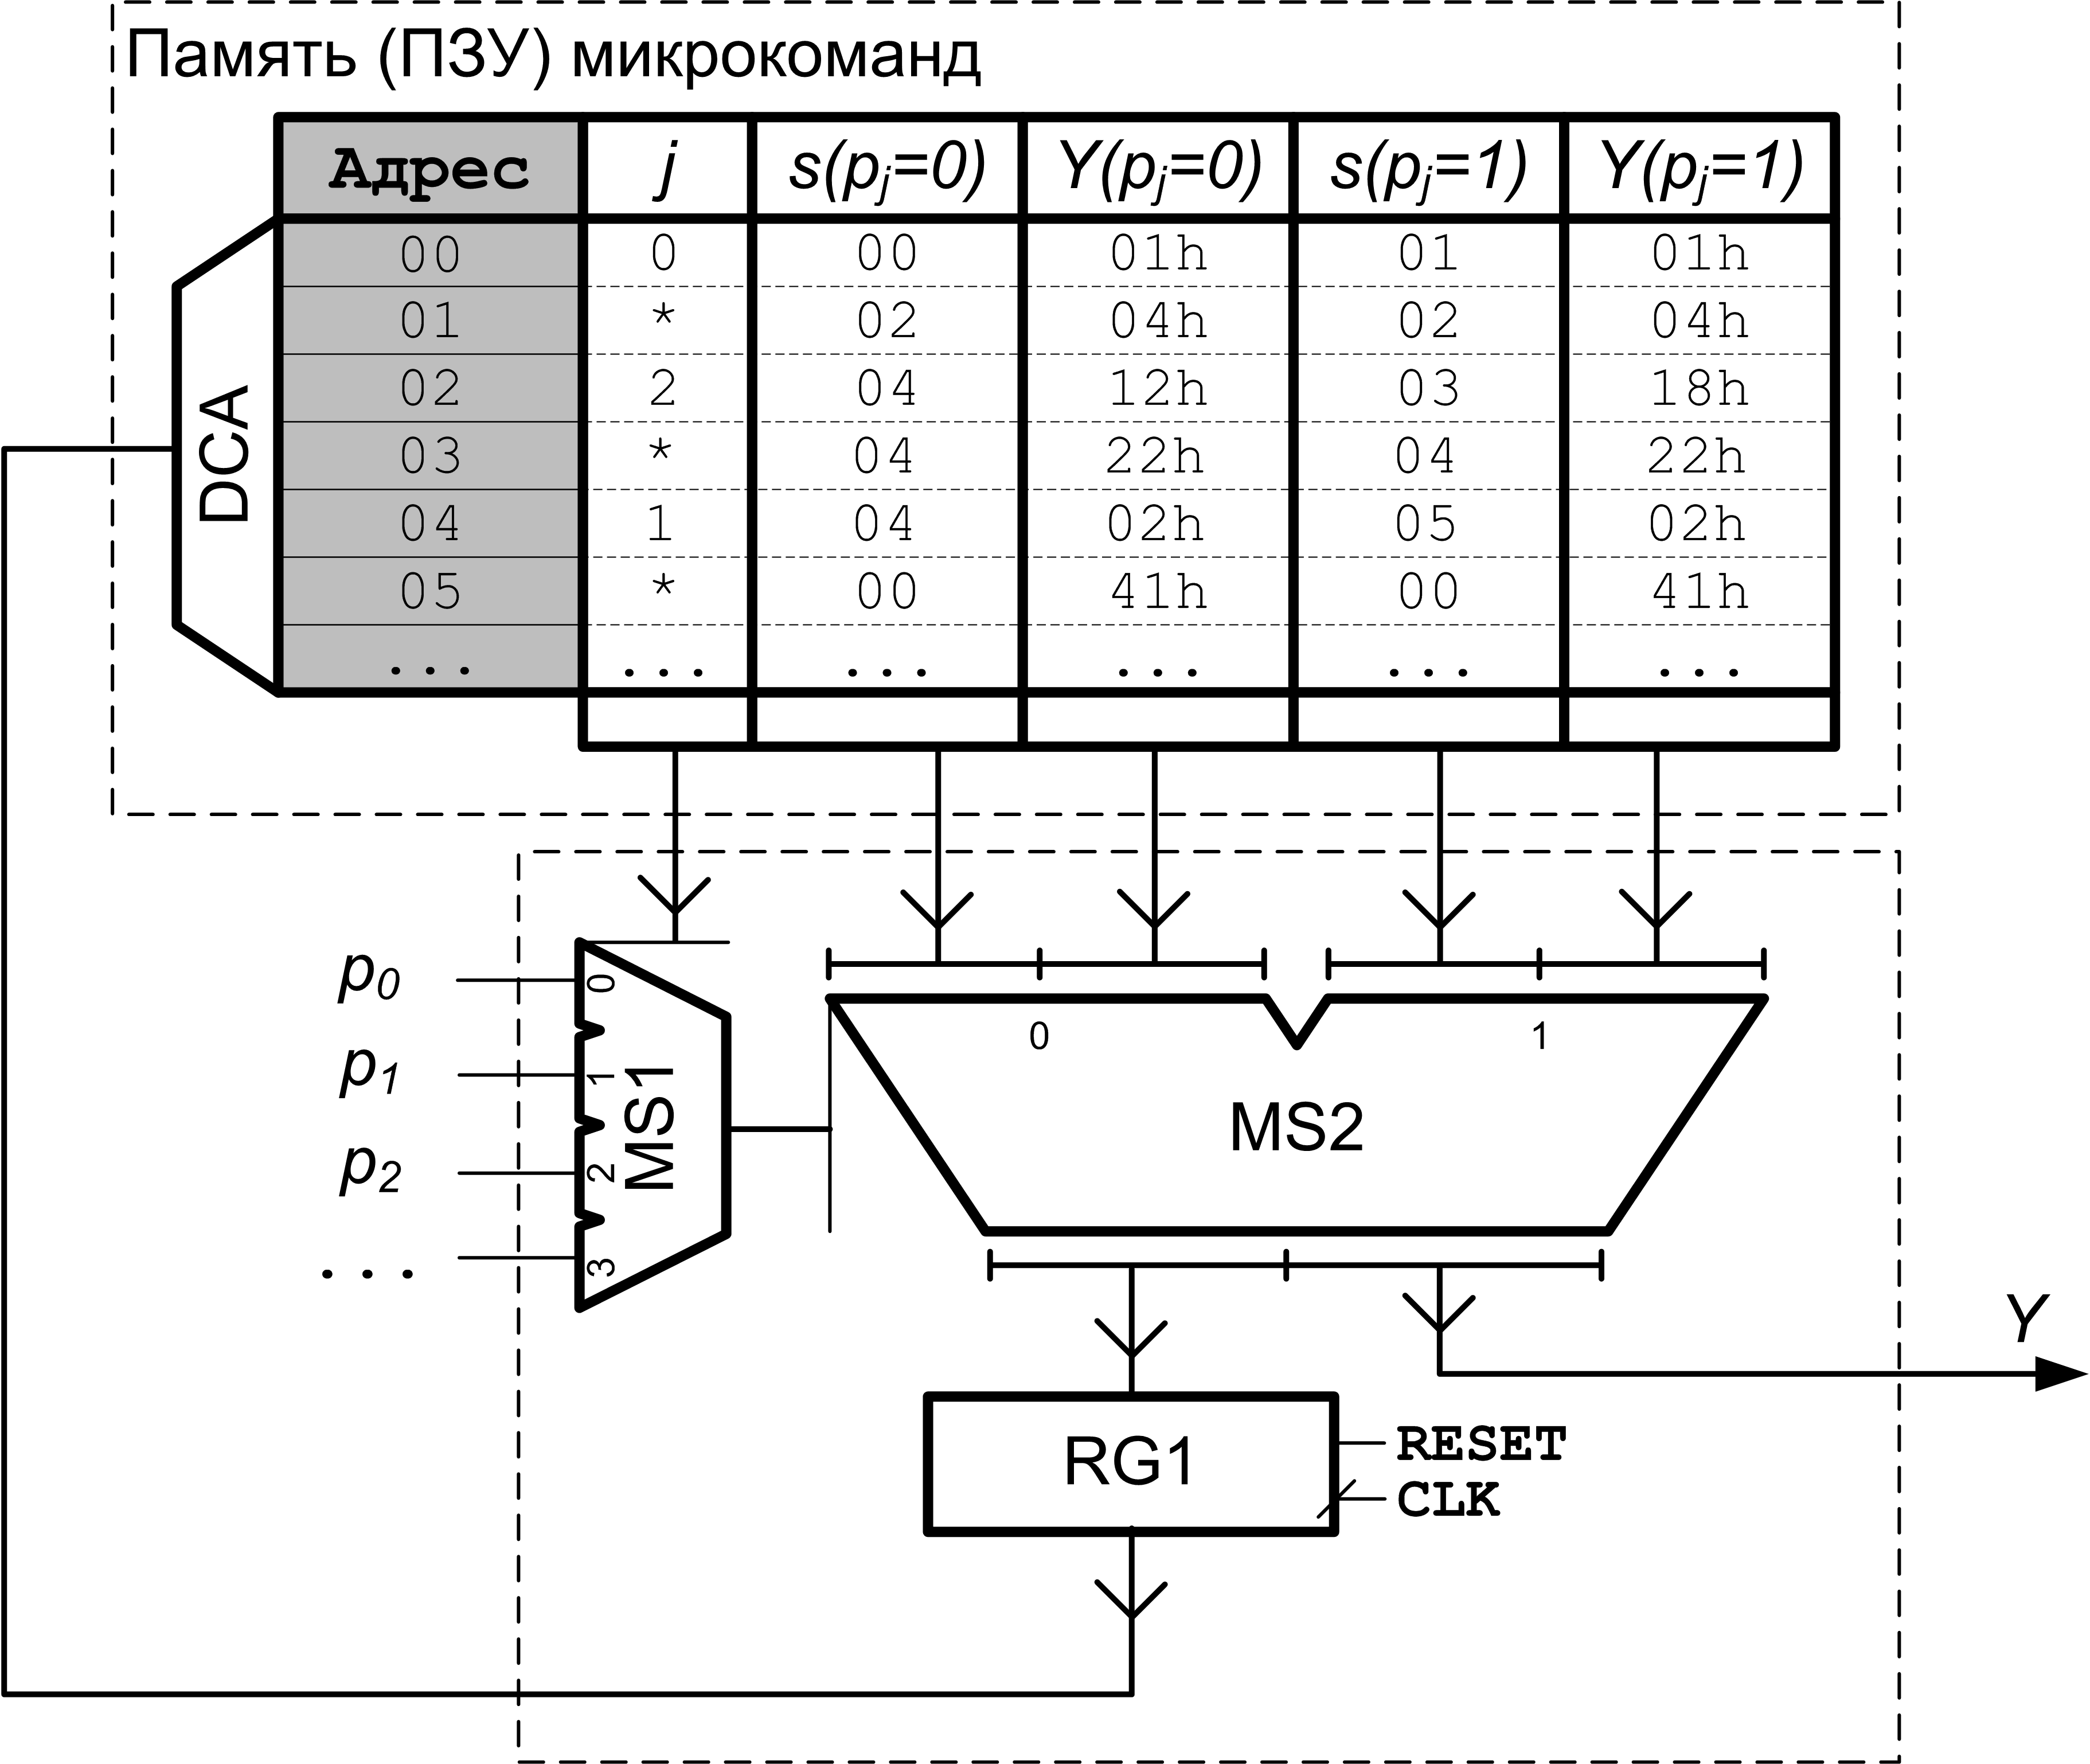
\includegraphics[width=.7\textwidth]{fig/miliMcu}
    \caption{Микропрограмма автомата Мили}
    \label{fig::ch::practice::miliMcu}
\end{figure}

Временная диаграмма работы преобразователя $\Machine{ПК}\mapsto\Machine{ДК}$ под управлением автомата Мили приводится на рисунке \ref{fig::ch::practice::timingsMili}.

\begin{figure}[!ht]
    \centering
    \includegraphics{fig/timings.3}
    \caption{Временная диаграмма работы преобразователя $\Machine{ПК}\mapsto\Machine{ДК}$ под управлением автомата Мили}
    \label{fig::ch::practice::timingsMili}
\end{figure}


\subsubsection{Автомат Мура}

Алгоритм работы преобразователя $\Machine{ПК}\mapsto\Machine{ДК}$, учитывающий особенности управляющего автомата Мура приведен на рисунке \ref{fig::ch::practice::moorePcDcAlgo}.

%todo особенности

\begin{figure}[!ht]
    \centering
    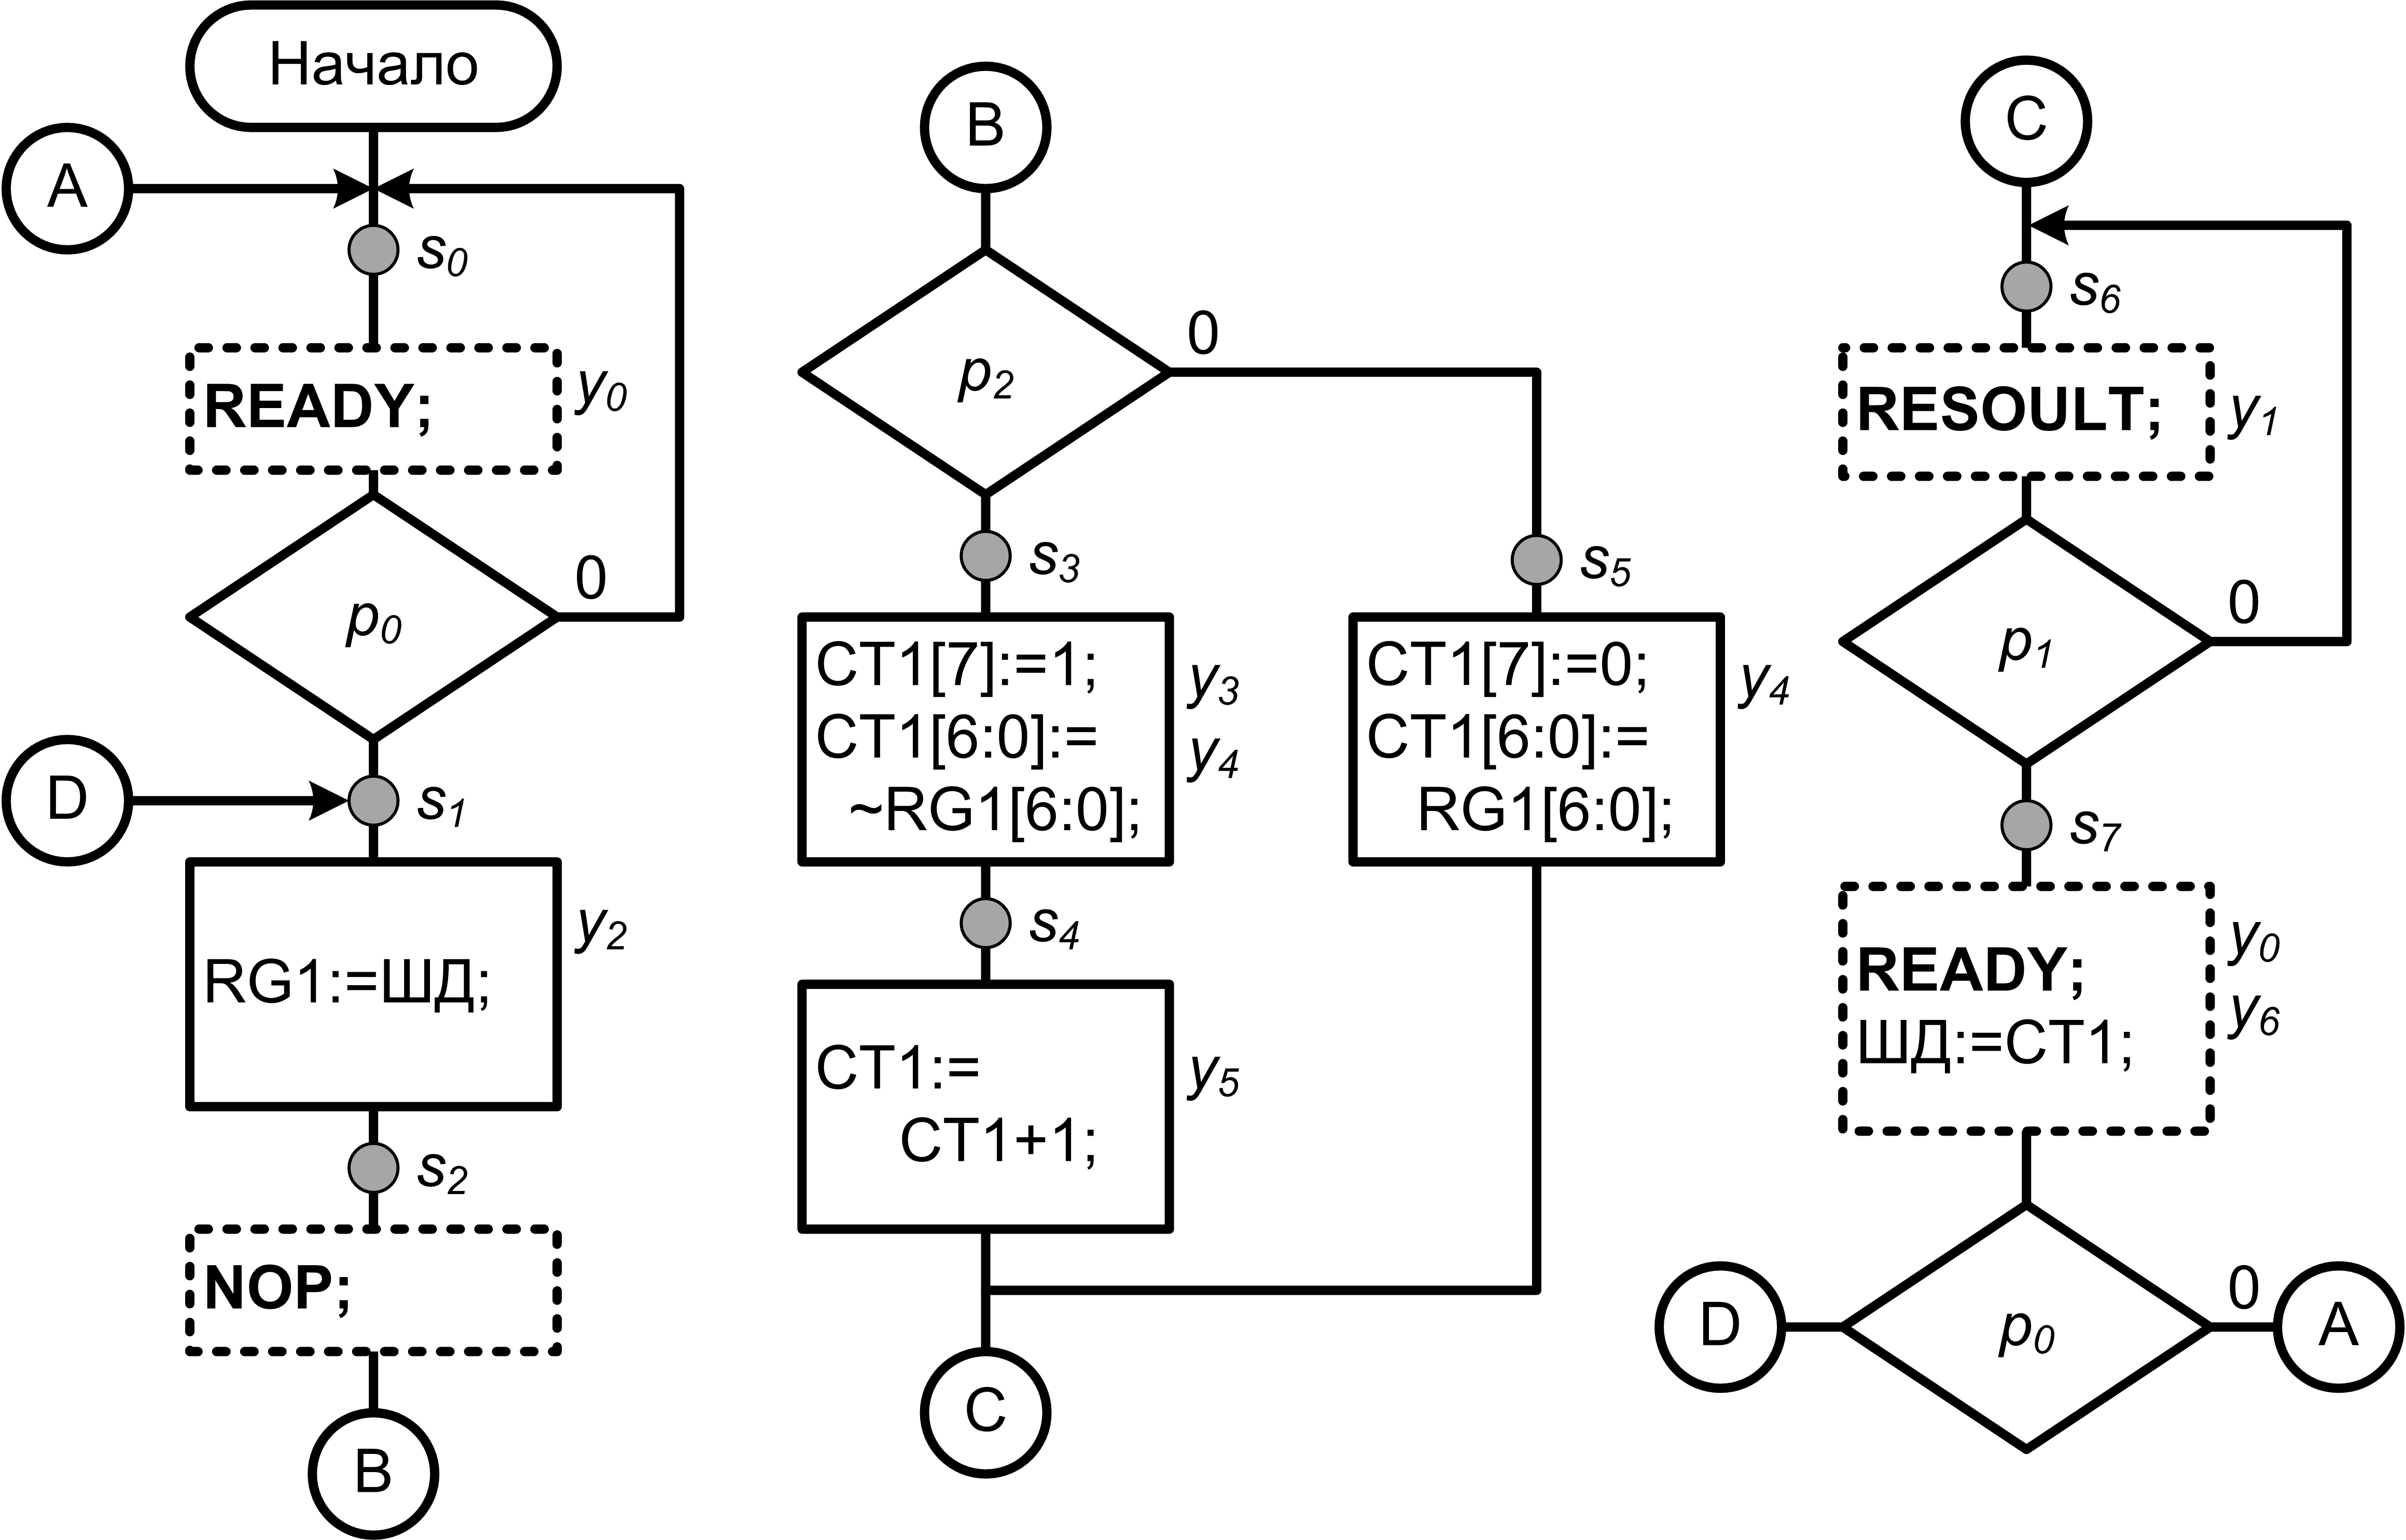
\includegraphics[width=\textwidth]{fig/moorePcDcAlgo}
    \caption{Алгоритм работы преобразователя $\Machine{ПК}\mapsto\Machine{ДК}$ под управлением автомата Мура}
    \label{fig::ch::practice::moorePcDcAlgo}
\end{figure}

Диаграмма состояний автомата Мура уже была приведена на рисунке \ref{fig::ch::practice::MooreDiagram}. Обычно у автомата Мура, эквивалентного автомату Мили, состояний больше, и времени (тактов) на работу он также тратит больше.

Прошивка памяти микропрограммного автомата Мура приводится на рисунке \ref{fig::ch::practice::mooreMcu}.

\begin{figure}[!ht]
    \centering
    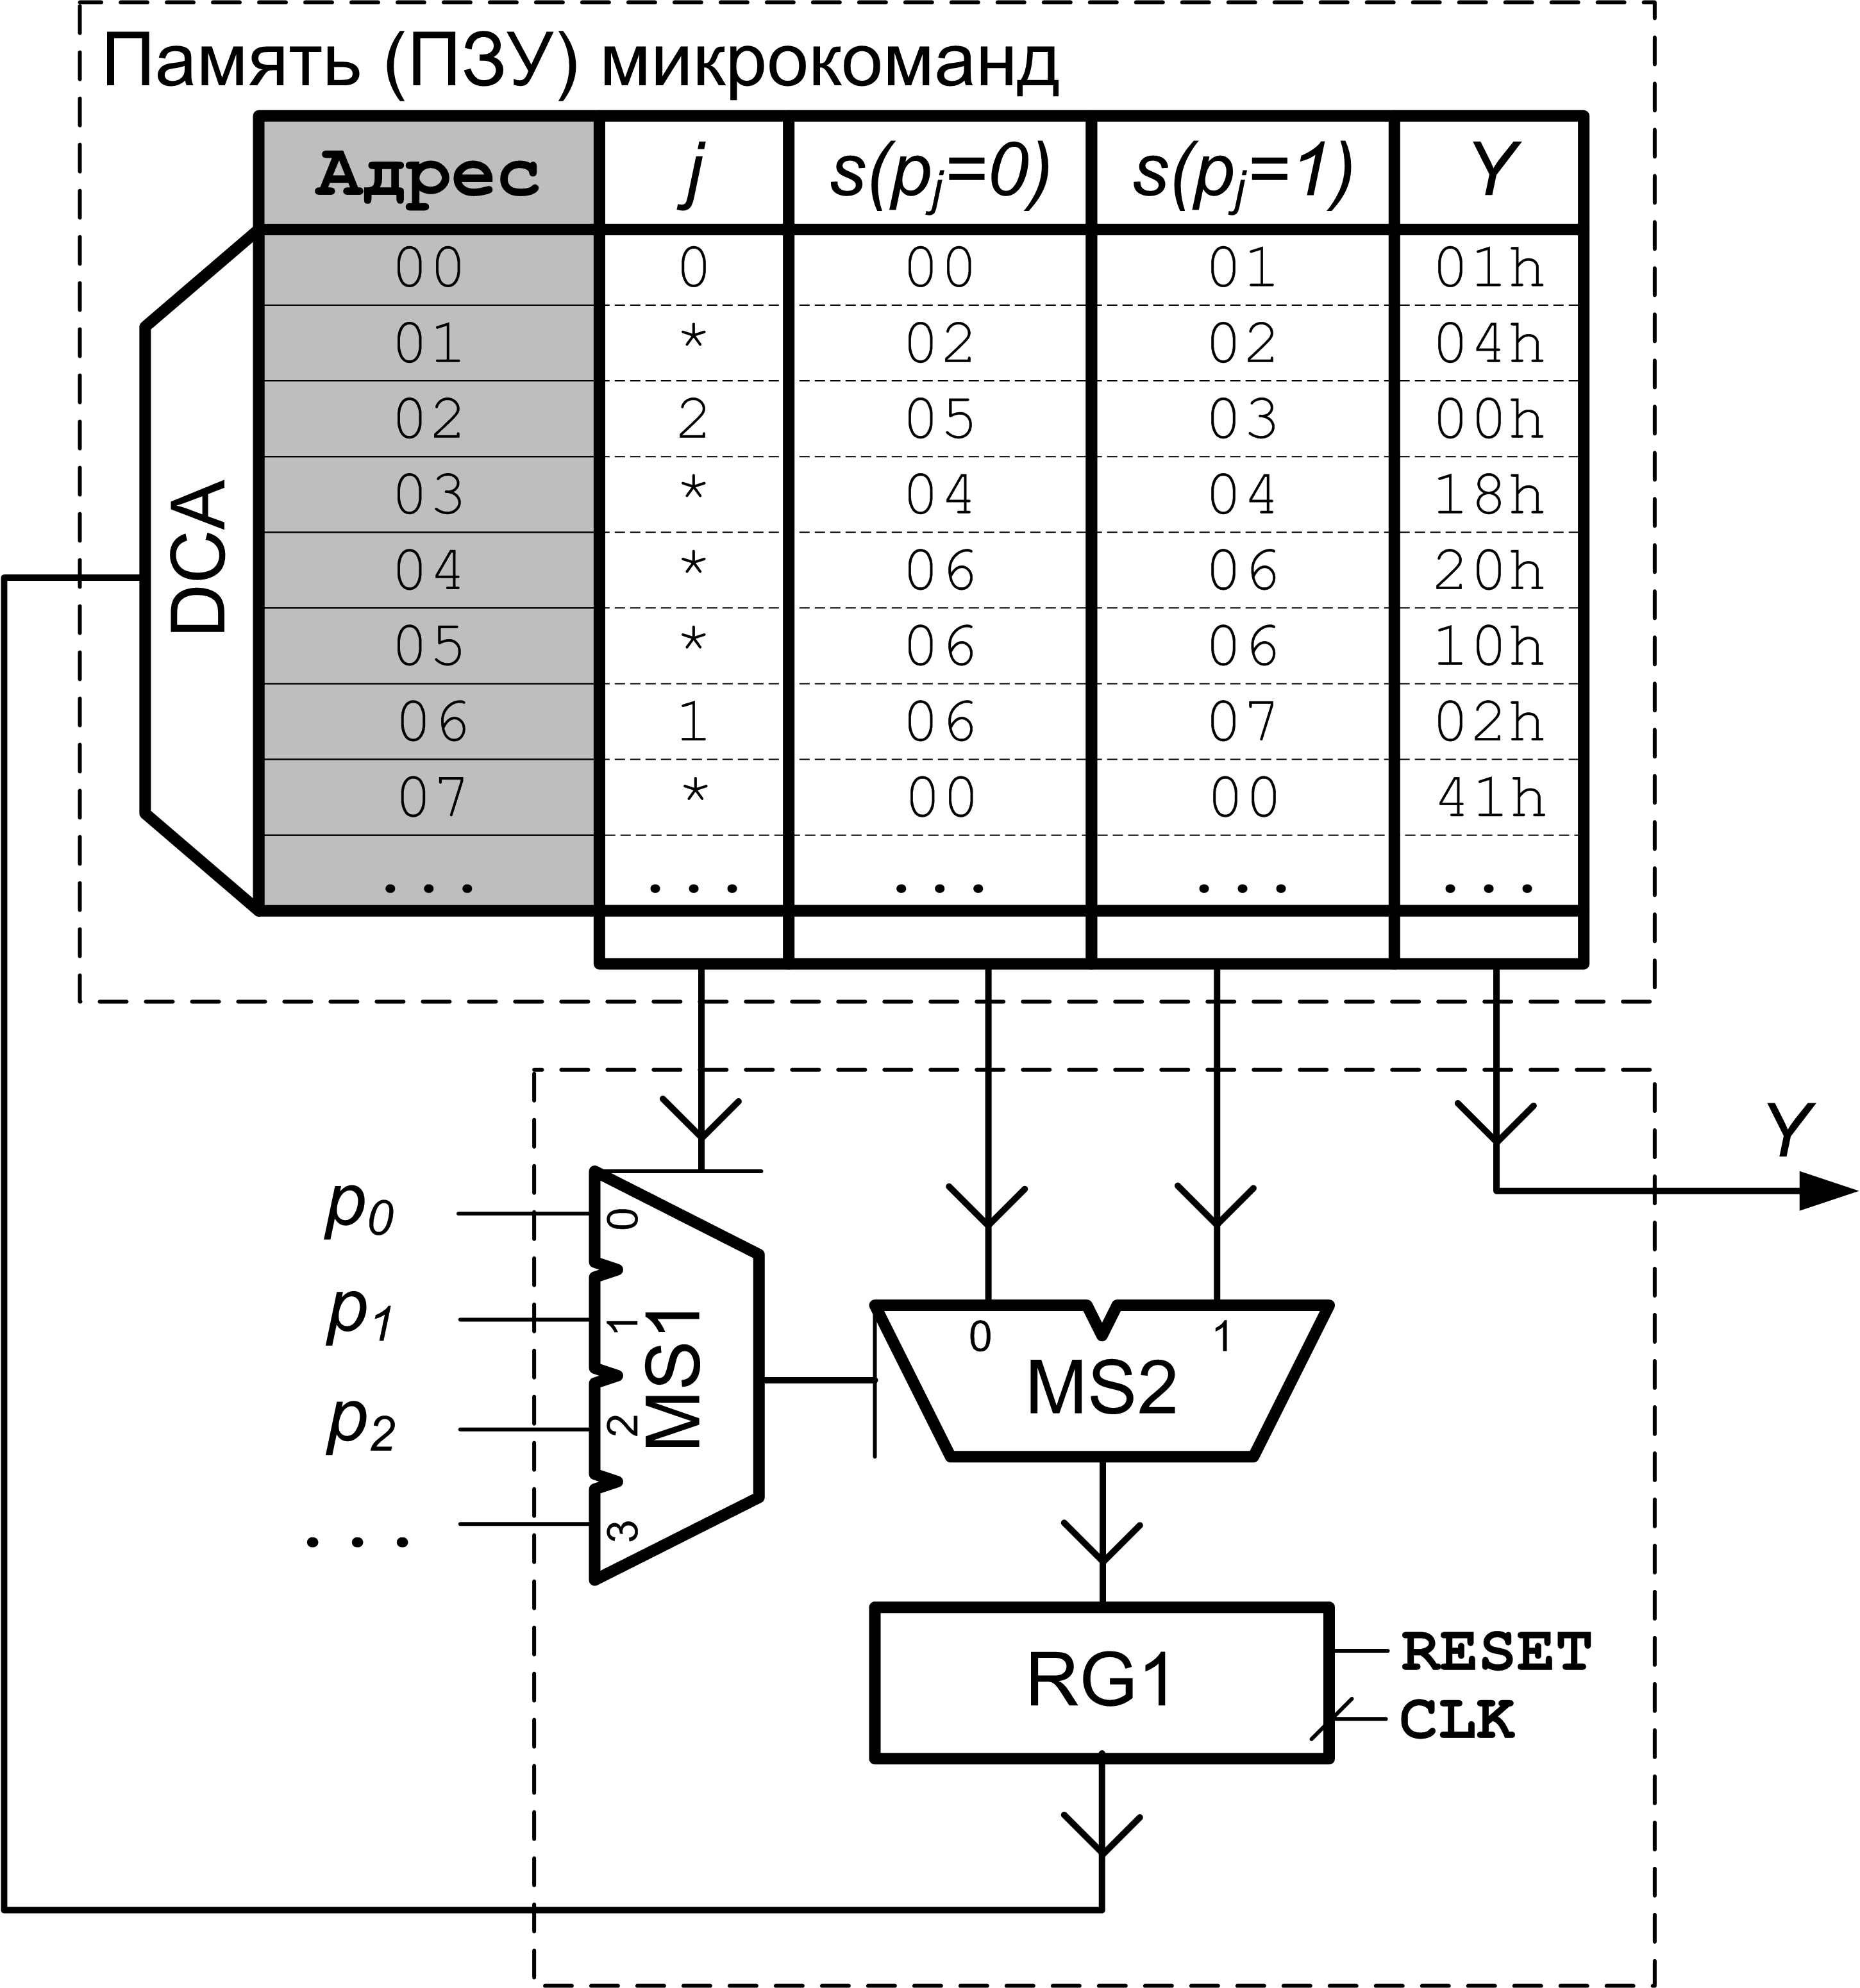
\includegraphics[width=.6\textwidth]{fig/mooreMcu}
    \caption{Микропрограмма автомата Мура}
    \label{fig::ch::practice::mooreMcu}
\end{figure}

Временная диаграмма работы автомата Мура приведена на рисунке \ref{fig::ch::practice::timingsMoore}.

\begin{figure}[!ht]
    \centering
    \includegraphics{fig/timings.4}
    \caption{Временная диаграмма работы преобразователя $\Machine{ПК}\mapsto\Machine{ДК}$ под управлением автомата Мура}
    \label{fig::ch::practice::timingsMoore}
\end{figure}


